\subsection{Introduction}
The implementation of static or adaptive grid refinement in global atmospheric general circulation models (AGCMs) is a desirable, and increasingly common feature of next-generation atmospheric models. Regional grid refinement permits the explicit simulation of processes at the kilometric scale in a global model, providing a unification of global, regional and, in some cases, cloud-scale weather and climate simulations within a single AGCM framework \citep[e.g.,][]{LETAL2001MWR,WA2011MWR,RETAL2013JCLIM,Z2014QJRMS,ZetAl2014JCb,RHUZ2016,HETAL2016JCLIM}. This framework permits the interaction of the refined region with the globally resolved circulation, resulting in an autonomous representation of energy and enstrophy cascades \citep{C1971JAS,L1999JFM}, and global teleconnections \citep{WG1981MWR} that may affect the solution locally. 

The spectral element dynamical core option (CAM-SE) in the Community Atmosphere Model (CAM) has been designed to support variable resolution grids \citep{ZetAl2014JCb,GetAl2014GMD}. While CAM-SE is equipped with higher order numerics and local conservation properties to prevent degradation of the solution across highly distorted elements \citep{TF2010JCP,ZetAl2014JC,GetAl2014GMD}, the resolved vertical motion and precipitation rates exhibit an alarming sensitivity to grid-refinement \citep[e.g.,][]{RETAL2012ASL,YETAL2014JCLIM,ZetAl2014JCb,OETAL2016JAMES,HR2017JCLIM}. Although it is commonly accepted that the sensitivity of AGCM solutions to grid-refinement are related to the parameterization of moist physics, the exact mechanisms are not clearly identified. The difficulties of deciphering causes of diverging AGCM solutions under grid-refinement lie in the significant complexity of the models themselves. For example, it is quite common for an AGCM to have three distinctly separate schemes for predicting cloud amount \citep[e.g.,][]{PETAL2014JCLIM}. While there may be satisfactory reasons for this separation, and not withstanding recent advances in unified cloud schemes \citep{GETAL2002JAS,P2014JAS}, this complexity makes it difficult to unravel which component of which scheme, or interactions with other parts of the model, are contributing to the model’s behavior. 

An alternative explanation for the resolution sensitivity observed in AGCMs relates to the inherent scale dependencies of the underlying equations of motion \citep{F2007JAS,HR2017JCLIM}. These scale dependencies have been discussed before in the context of non-hydrostatic convection permitting simulations \citep{O1981JAS,WETAL1997MWR,PG2006JAS,JR2016QJRMS}, but its relevance to hydrostatic convection in AGCMs is rarely discussed \citep{F2007JAS,J2017JAMES}. This is hardly surprising since convection schemes are implemented in AGCMs to reduce the occurrence of resolved convection, and may lead many to question whether resolved convection occurs in AGCMs at all. However, evidence showing the importance of resolved updrafts and downdrafts on simulated tropical convective systems in AGCMs can be found as far back as \cite{MK1997QJRMS}, and more recently by \cite{OETAL2016JAMES}.

\begin{figure}[t]
\begin{center}
\noindent\includegraphics[width=25pc,angle=0]{chapter3/Figure1.eps}\\
\end{center}
\caption{Instantaneous snapshot of the vertical pressure velocity (colors) and the diabatic forcing from the column physics (black contours) for a longitude-height transect at the equator from a series of aqua-planet simulations at four different horizontal resolutions. Contour interval is $+10$ K day$^{-1}$ (solid) and $-10$ K day$^{-1}$ (dashed).}
\label{fig:figure3-1}
\end{figure}

Figure~\ref{fig:figure3-1} illustrates the prevalence of resolved updrafts in an AGCM. The simulations are from a series of CAM-SE aqua-planet simulations \citep[following][]{NH2000ASL} at four different horizontal resolutions typical of present day AGCMs. The only parameters varied in the simulations are the dynamics time-step and hyper-viscosity coefficients, and the physics time-step is set to 1800 s for all resolutions (Table~\ref{tbl:table3-1}). All other aspects of the simulations are identical to the aqua-planet reference simulation described in \cite{MWO2016JAMES}. Instantaneous snapshots of the vertical pressure velocity in the longitude-pressure plane at the equator for four different quasi-uniform horizontal resolutions are overlain by contours of large-magnitude, instantaneous diabatic forcing from the column physics. Resolved updrafts and downdrafts, primarily a response to grid-scale ``thermals" and re-evaporation of falling condensate by the large-scale condensation scheme, populate the deep tropics and are a crucial component of the tropical circulation \citep{HR2017JCLIM}. 

What is also clear from Figure~\ref{fig:figure3-1} is that the magnitude of the vertical motion, as well as the horizontal scale of the diabatic forcing and resolved convective elements as a whole, has some proportional relation to the grid spacing. The global power spectrum of the diabatic forcing arising from the column physics in the simulations (Supplementary Figure~\ref{fig:sfigure3-1}) provides conclusive evidence for a reduction in diabatic forcing scale with resolution. As discussed in \cite{HR2017JCLIM}, the relationship between the horizontal scale of the buoyancy forcing, and the magnitude of the vertical velocity is consistent with the equations of motion. To illustrate this point, we proceed with a scale analysis of the non-rotating, dry equations of motion in the anelastic framework described in \cite{JR2016QJRMS}.

\cite{JR2016QJRMS} augment the conventional anelastic approximation with a few important modifications. The first modification is that the full pressure is split between a locally balanced hydrostatic pressure, $p_{HYD}$, and a non-hydrostatic residual \citep{D1979JAS}. The second modification is the introduction of the effective buoyancy, $\beta$. The effective buoyancy is the vertical acceleration that would result from zeroing out the wind field, which is useful for isolating the component of vertical acceleration due to the Archimedean buoyancy. \cite{JR2016QJRMS} then introduce the buoyancy pressure, $p_{\beta}$, which is the residual non-hydrostatic pressure associated with zeroing out the wind field, the vertical gradient of which is the effective buoyancy. These modifications lead to the Poisson equation \citep[equation 8 in][]{JR2016QJRMS}:
\begin{equation}
-\nabla (p_{\beta}) = \nabla^{2}_{h} (p_{HYD}),\label{eq:eq3-1}
\end{equation} 
where $\nabla^2$ is the Laplacian operator ($\nabla^{2}_{h} + \frac{d^2}{dz^2}$) and $\nabla^{2}_{h}$ is ($\frac{d^2}{dx^2} + \frac{d^2}{dy^2}$). Consider a vertical column of air of diameter $D$ and height $H$, and constant Archimedean buoyancy $B_0$ throughout, then after taking the vertical derivative of equation~\ref{eq:eq3-1}, the scale analysis for $\beta$ is: 
\begin{equation}
\beta = B_0 \left[ D^2 \left( \frac{1}{D^2} + \frac{1}{H^2} \right) \right]^{-1},\label{eq:eq3-2}
\end{equation}
\citep[compare to equation 10 in][]{JR2016QJRMS}. Setting the scale of $\beta$ to $W/T$, where $W$ is a vertical velocity scale and $T=H/W$, and noting that at hydrostatic scales $\frac{1}{D^2}  \ll \frac{1}{H^2}$, solving for $W$:
\begin{equation}
W = \sqrt{B_0 H} \frac{H}{D}. \label{eq:eq3-3}
\end{equation}
The vertical velocity scale due to the Archimedean buoyancy is inversely proportional to the horizontal scale of the Archimedean buoyancy, at hydrostatic scales. Inspection of the Poisson equation (equation~\ref{eq:eq3-1}) indicates that the $1/D$ scaling is a result of the horizontal scale of the hydrostatic pressure perturbation, which drives convergence into the air column and vertical motion. The horizontal scale of the hydrostatic pressure perturbation is set by the horizontal scale of the Archimedean buoyancy \citep{JR2016QJRMS}, and determined by the horizontal scale of the diabatic forcing.

Through assuming a linear relationship between grid spacing ($\Delta x$) and diabatic forcing scale, which remains untested, but which \cite{J2017JAMES} has shown evidence for at cloud-permitting resolutions, one may expect the variations in vertical velocity to go like $\Delta x^{-1}$. However, a $\Delta x^{-1}$ relationship, while consistent with the general trend of greater vertical motion at higher resolution (e.g. Figure~\ref{fig:figure3-1}), overestimates the resolution sensitivity observed in a series of CAM-SE aqua-planet simulations analyzed in \cite{HR2017JCLIM}. The simulations depicted in Figure~\ref{fig:figure3-1} are similar – the  $\Delta x^{-1}$ scaling overestimates the sensitivity to horizontal resolution (Figure~\ref{fig:figure3-10}, dashed lines). The $\Delta x^{-1}$ scaling may be incorrect simply because the relationship between diabatic forcing scale and $\Delta$ is non-linear. Alternatively, through maintaining the linear relationship between forcing scale and $\Delta x$, \cite{HR2017JCLIM} propose that feedbacks within other components of the AGCM steer the solution towards a weaker resolution sensitivity.
 
The goal of this paper is to test the robustness of the scaling (equation~\ref{eq:eq3-3}) in a simplified, non-rotating AGCM framework. We begin with an idealized set of rising thermal bubbles using CAM-SE without moist processes, and incrementally introduce some moist parameterizations to determine how their inclusion may affect the scaling of equation~\ref{eq:eq3-3}. We do not consider the influence of convection schemes – CAM convection schemes are incompatible with our experimental design. While this limits our ability to extend our results to the behavior of a complete AGCM, we argue that our simplified moist framework is still relevant to the behavior of a complete AGCM, and as such, will shed light on whether the moist physics or the scale dependencies of the dry equations of motion are the driving force behind the resolution sensitivity in CAM. 

\begin{table}
\begin{center}
\noindent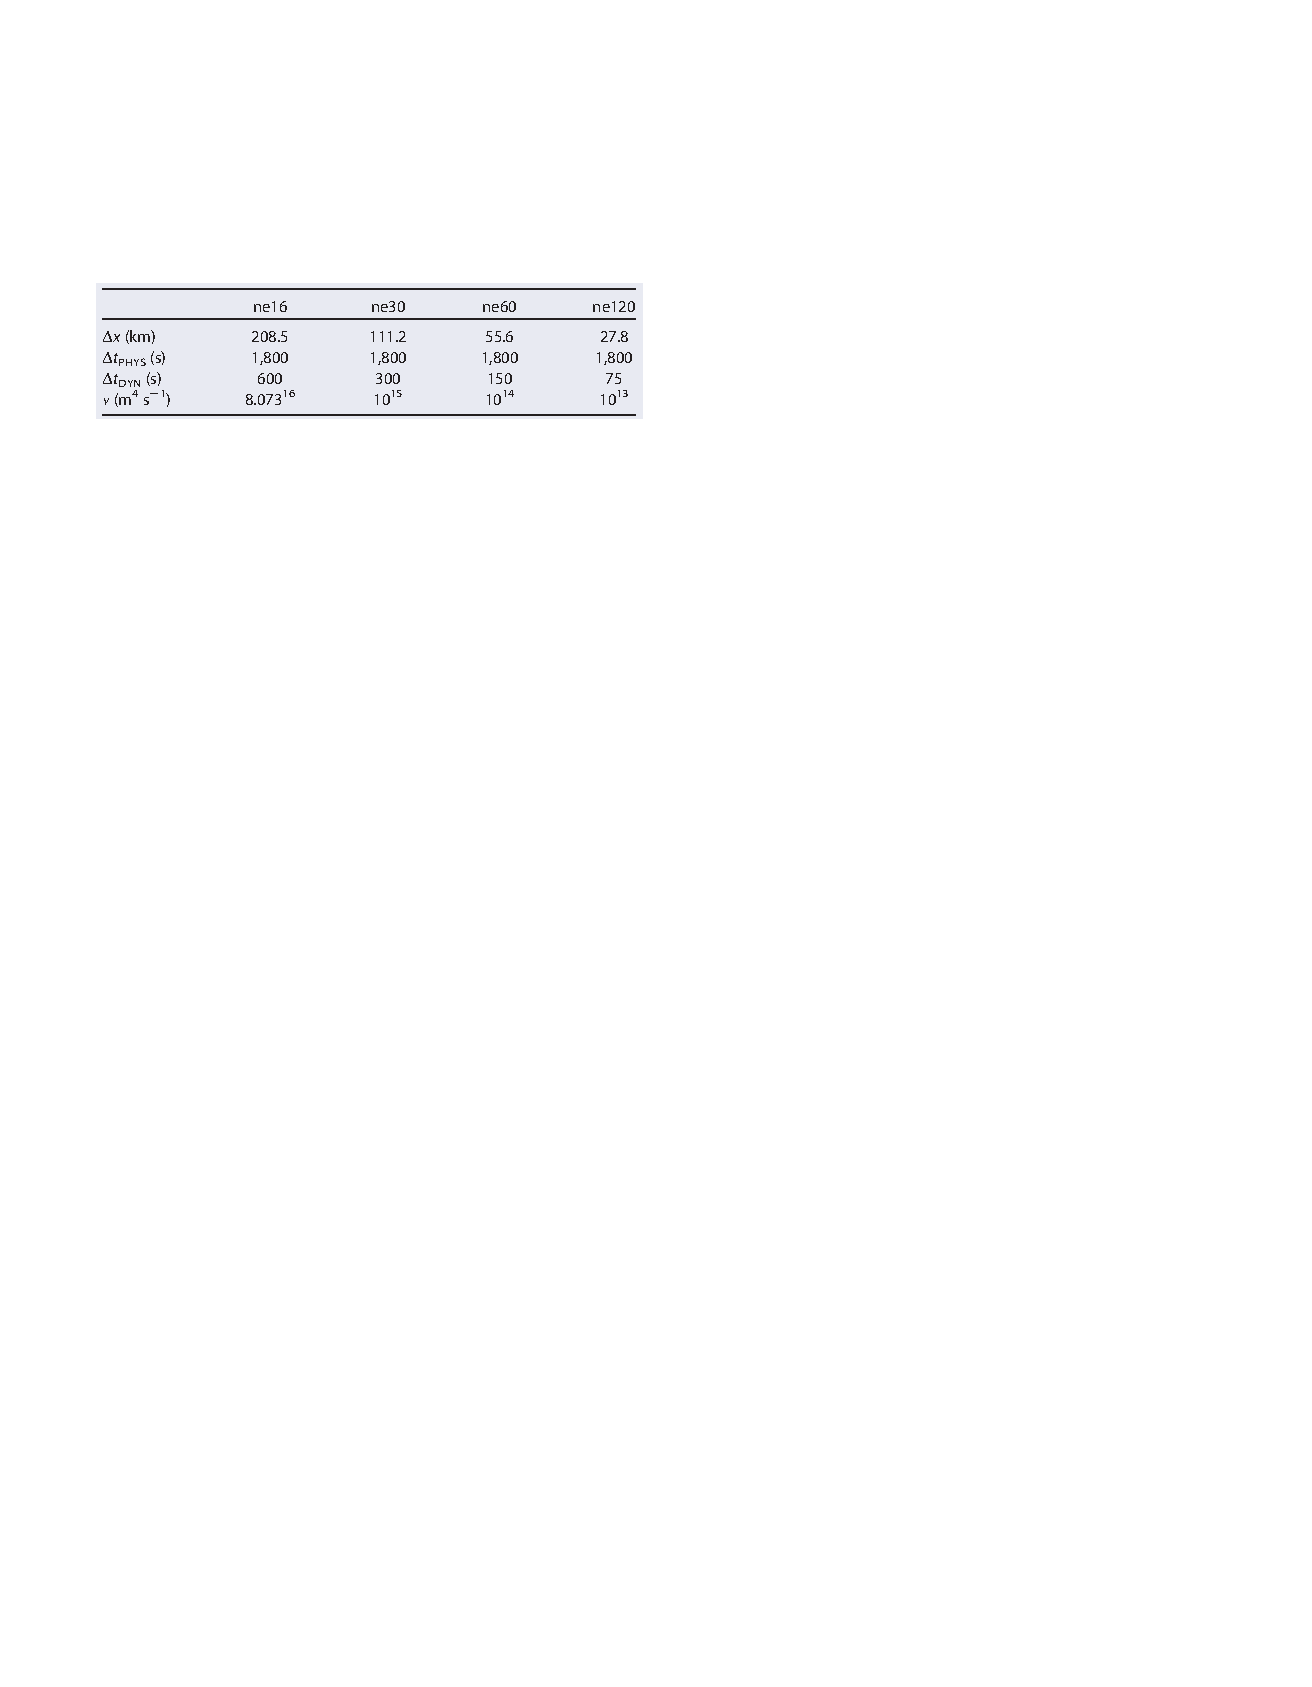
\includegraphics[width=25pc,angle=0]{chapter3/table1.pdf}\\
\end{center}
\caption{Quasi-uniform horizontal grid spacing ($\Delta x$), time-stepping ($\Delta t$) and hyper-viscosity coefficients ($\nu$) used in the aqua-planet simulations. Hyper-viscosity coefficients are after \cite{ZetAl2014JC} and are identical for the treatment of momentum, temperature and specific humidity.}
\label{tbl:table3-1}
\end{table}

Rising bubble experiments are commonly used to test atmospheric models, although they are disproportionately used in non-hydrostatic models, often resembling an idealized thermal with horizontal scales on the order of a kilometer or less \citep{KW_1978JAS,GETAL1991JAS,BETAL2002MWR,JR2016QJRMS}. The focus of this study is on bubbles of hydrostatic scale, and are intended as a surrogate grid-scale thermal occurring in more complex AGCM configurations (e.g., Figure~\ref{fig:figure3-1}). Section 3.2 provides an overview of the dynamical cores and moist physical parameterizations used throughout the paper, and a description of the analytical initial conditions. Section 3.3 presents the results of the experiments, Section 3.4 contains a discussion of the results and section 3.5 provides some concluding thoughts.

\subsection{Materials and Methods}
\subsubsection{Dynamical Cores}
For most of our experiments, we choose to work with the spectral element dynamical core option of the Community Atmosphere Model \citep[CAM-SE;][]{DetAl2012IJHPCA}, the atmospheric component of the Community Earth System Model, version 1.2. CAM-SE solve the vector-invariant hydrostatic primitive equations using a fourth-order accurate, continuous Galerkin method on the sphere. A brief overview of the CAM-SE dynamical core is provided in \cite{HR2017JCLIM}, and further details are available in the model documentation \citep{CAM5}. The version of CAM-SE used in this study is more recent than for the simulations analyzed in \cite{HR2017JCLIM}, with the main distinction being the change to a third-order accurate, five-stage Runge Kutta time-stepping scheme \citep{DetAl2012IJHPCA,GU2016GMD}.

CAM-SE uses an unstructured, cubed-sphere grid. For the quasi-uniform grid used in this study, the notation for the cubed-sphere grid is abbreviated by the number of elements along the edge of one of the six cubed-sphere panels. The grid used in this work contains 30 elements along the edge of a cubed-sphere face (abbreviated as ‘ne30’). Since each element contains 4 interior Gauss-Lobatto-Legendre (GLL) quadrature nodes, and 12 GLL nodes along the (shared) element boundary, the ne30 simulations correspond to an average horizontal grid-spacing of 111.2 km. The CAM-SE dynamical core contains no implicit dissipation in the horizontal, and so fourth-order hyper-viscosity operators are applied to state variables to suppress numerical artifacts \citep{DetAl2012IJHPCA}. The resolution dependent hyper-viscosity coefficients used throughout this study are the same as those used for the aqua-planet experiments provided in Table~\ref{tbl:table3-1}, and are from \cite{ZetAl2014JC}.

Experiments are also performed using the finite-volume dynamical core in CAM \citep[CAM-FV;][]{L2004MWR,CAM5}. CAM-FV solves for the horizontal dynamics using a finite-volume formulation of the vector invariant primitive equations \citep{LR1997QJR}. Like CAM-SE, CAM-FV utilizes the “Vertically Lagrangian” method \citep{L2004MWR}, solving the horizontal dynamics within floating hybrid sigma-pressure surfaces, and periodically remapping the state back to a Eulerian, vertical reference coordinate \citep{CAM5}. CAM-FV contains implicit dissipation of scalars quantities, which includes vorticity, and explicit divergence damping is applied to the divergent winds. Both CAM-SE \citep{DetAl2012IJHPCA}, and CAM-FV \citep{L2011IJHPC,WJRL2010MWR} contain default fourth-order divergence damping, but to promote a larger diversity in design choices between the two dynamical cores, the second-order divergence damping option is used in CAM-FV \citep{CAM3}. However, sensitivity experiments will be discussed that quantify the effect of the order of the divergence damping operator in CAM-FV. The dynamics are solved on a latitude-longitude grid, and necessitates a polar filter to stabilize solutions in polar regions \citep{CAM5}. A standard grid with a horizontal resolution of $0.9^{\circ}$ latitude by $1.25^{\circ}$ longitude (nominally $1^{\circ}$), equivalent to an average equatorial grid spacing of 139 km, is used in all CAM-FV experiments.

The vertical resolution is the same for all grids in this study (regardless of dynamical core), consisting of 30 unequally spaced, hybrid sigma-pressure levels \citep{CAM5}. Higher horizontal resolution grids are obtained by reducing the Earth-like planetary radius to match the resolution of other grid configurations, as in \cite{RM2016GRL}. Modifications to the Coriolis parameter are not required - only non-rotating planets are considered in this study. For all experiments described in this paper, a dynamics time-step of 75 seconds and 56.26 seconds are used in CAM-SE and CAM-FV, respectively, which satisfy the stability constraints of the highest resolution grids used throughout the study. The motivation for fixing the dynamics time-step, regardless of horizontal resolution, is in part for simplicity, but also to generalize our results to the behavior of the variable resolution version of CAM-SE. The variable resolution version of CAM-SE requires the time-step to be equal everywhere on the grid, and must be chosen to satisfy the Courant number in the refined region \citep{ZetAl2014JC}.

\subsubsection{Moist Physics}
The moist experiments contain water species and parameterizations of moist processes. Water species are transported by the dynamical core, and the parameterizations are computed at the end of every third dynamics time-step in CAM-SE, and every fourth dynamics time-step in CAM-FV, equivalent to a physics time-step of 225 s. Further details on the coupling of the dynamical cores to the physical parameterizations is described in \cite{HR2017JCLIM} and \cite{CAM5}. We experiment with parameterizations that are intended to span the spectrum of complexity. In the least complex case, the dynamical cores are coupled to the large-scale condensation scheme of the ‘simple physics’ package of \cite{RJ2012JAMES}, which we refer to as ‘simple condensation’ throughout the manuscript. This warm-rain scheme assumes all condensates are immediately removed from the column with no cloud phase.

Towards the other end of the spectrum, the Community Atmosphere Model, version 5 physics package \citep[CAM5;][]{CAM5} contains a stratiform cloud scheme, with separate macrophysical \citep{PETAL2014JCLIM} and microphysical \citep{MG2008JC} routines that together, constitute a more complex large-scale condensation scheme. The stratiform scheme computes ice and liquid cloud phases through prognostic equations for cloud droplet number and concentration, and contains an explicit representation of falling hydrometeors \citep{MG2008JC}. As in the aqua-planet reference simulations presented in \cite{MWO2016JAMES}, the cloud liquid and cloud ice concentrations are held to constant values ($100 \times 10^6$ m$^{-3}$ and $0.1 \times 10^6$ m$^{-3}$, respectively) to suppress dependencies on aerosol species, which are not present in our simulations. As a final level of complexity, we couple the stratiform scheme with the downgradient vertical dissipation routine used in CAM5 for the free troposphere, which diffuses momentum, temperature and specific humidity using standard mixing length and Richardson number dependent formulations \citep{CAM4}.

\begin{figure}
\begin{center}
\noindent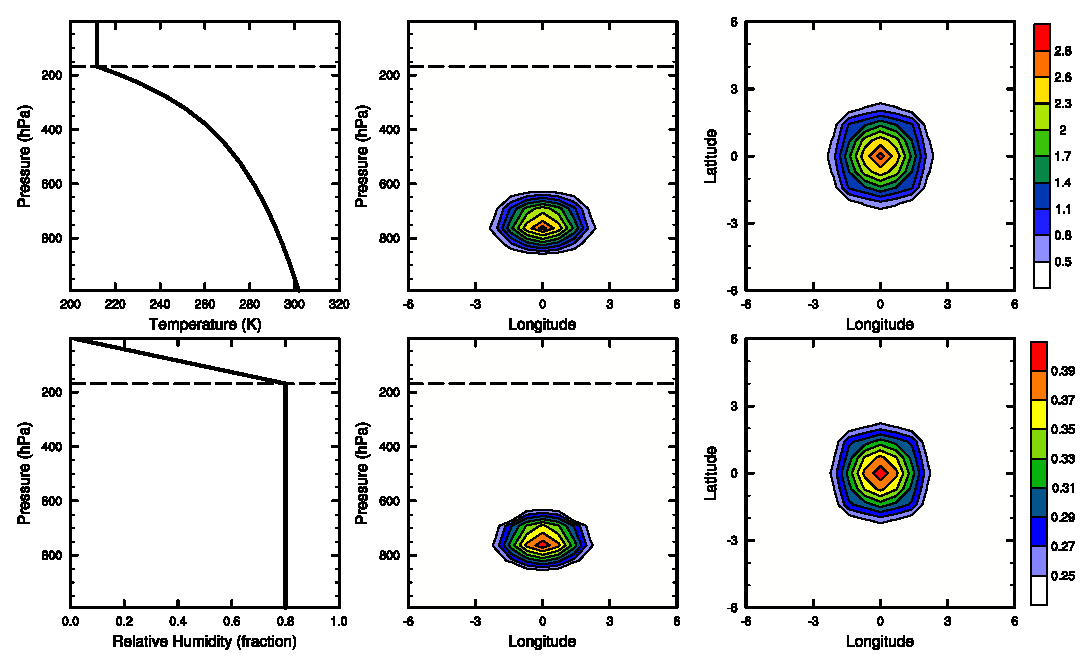
\includegraphics[width=25pc,angle=0]{chapter3/Figure2.eps}\\
\end{center}
\caption{Initial conditions used in the moist experiments. Background temperature (top, left) and background relative humidity (bottom, left) reference profiles.  A moist bubble with $r_h = X \times 350$ km, where $X$ is the scale factor from Table~\ref{tbl:table3-2}, is depicted in the middle and right plots: potential temperature perturbation in the longitude-pressure plane (top, middle) and the latitude-longitude plane (top, right) and the relative humidity perturbation in the longitude-pressure plane (bottom, middle) and the latitude-longitude plane (bottom, right). The horizontal dashed lines denotes the location of the tropopause.}
\label{fig:figure3-2}
\end{figure}

\subsubsection*{Initial Conditions}
The experiments are designed to isolate the scale sensitivity expressed in complex, moist AGCM resolution experiments, such as in Figure~\ref{fig:figure3-1}. The general procedure is to produce a set of approximately one-day long simulations of a rising thermal bubble in an idealized tropical environment, each bubble having its horizontal radius, $r_h$, and model horizontal grid-spacing, $\Delta x$, simultaneously reduced by a proportionality factor, $X$, to be defined later. An implicit assumption of this experimental design is that the forcing scale, $2 r_h$, is linear in $\Delta x$. 

The background temperature and moisture profiles are inspired by the thermodynamic structure of strongly convecting regions in the deep tropics of the aqua-planet simulations, and are similar to the neutrally stable conditions proposed by \cite{BETAL2002MWR}. The background temperature profile is a horizontally uniform, reversible moist adiabat pertaining to a surface temperature, $T_0$, and constant relative humidity with height, $h_0$. The tropopause pressure is the hydrostatically balanced pressure corresponding to a fixed height of 15 km, above which the temperature and specific humidity are set to the tropopause values (Figure~\ref{fig:figure3-2}).

A temperature perturbation is introduced following \cite{KETAL2015JAMES}:
\begin{equation}
T^{\prime} (R) = \begin{cases} \Delta \theta * \Pi * \cos^2 (R \frac{\pi}{2}) \: for \: R \leq 1 \\
						0 \; \; \; \; \; \; \; \; \; \; \; \; \; \; \; \; \; \; \; \; \; \; \; \; \; \; \; for \:R > 1 \end{cases}, \label{eq:eq3-4}
\end{equation}
with magnitude $\Delta \theta$. $\theta$ is the potential temperature, $\Pi = (p/p_0)^{\kappa}$ is the exner function and $\kappa = R_d/c_{pd}$, where $g$ is the gravitational acceleration, $R_d$ is the gas constant for dry air, $c_{pd}$ is the specific heat capacity of dry air at constant pressure and $p$ is the pressure. 
\begin{equation}
R(r,z) = \left[ \left( \frac{r}{r_h} \right)^2 + \left( \frac{z-z_c}{r_z} \right)^2 \right]^{\frac{1}{2}}, \label{eq:eq3-5}
\end{equation}
where $r_h$ is again the horizontal bubble radius, $r_z$ the vertical radius. The great circle distance, $r$ , from central latitude $\phi_c$ and central longitude  $\lambda_c$ is
\begin{equation}
r(\phi_c, \lambda_c) = a * \cos^{-1} \left( \sin(\phi_c) \sin(\phi) + \cos(\phi_c) \cos(\phi) * \cos(\lambda - \lambda_c) \right), \label{eq:eq3-6}
\end{equation}
where $a$ is the planetary radius. The hydrostatically balanced reference height, $z$, is found through vertical integration of the hydrostatic relation, and $z_c$ is the location of the bubble center in the vertical. A relative humidity perturbation is collocated with the temperature perturbation, and is of the form:
\begin{equation}
RH^{\prime} (R) = \begin{cases} \left( 1 - h_0 \right) + \Delta h * \Pi * \cos^2 (R \frac{\pi}{2}) \: for \: R \leq 1 \\
						0 \; \; \; \; \; \; \; \; \; \; \; \; \; \; \; \; \; \; \; \; \; \; \; \; \; \; \; \; \; \; \; \; \; \; \; \; \; \; \; \; \; \; \; \; for \:R > 1 \end{cases}, \label{eq:eq3-7}
\end{equation}
where $\Delta h$ is the magnitude of the relative humidity perturbation above saturation. The relative humidity parameters are set to $h_0 = 0.80$ and $\Delta h  = 0.20$ (relative humidity is defined as a fraction as opposed to a percent, throughout this work) modeled after the aqua-planets. The definition of relative humidity in the initial conditions needs to be made consistent with the parameterization one is using. The simple condensation scheme and the CAM5 physics package use different definitions for saturation vapor pressure, and their initial conditions were made consistent with these definitions.

\begin{table}
\begin{center}
\noindent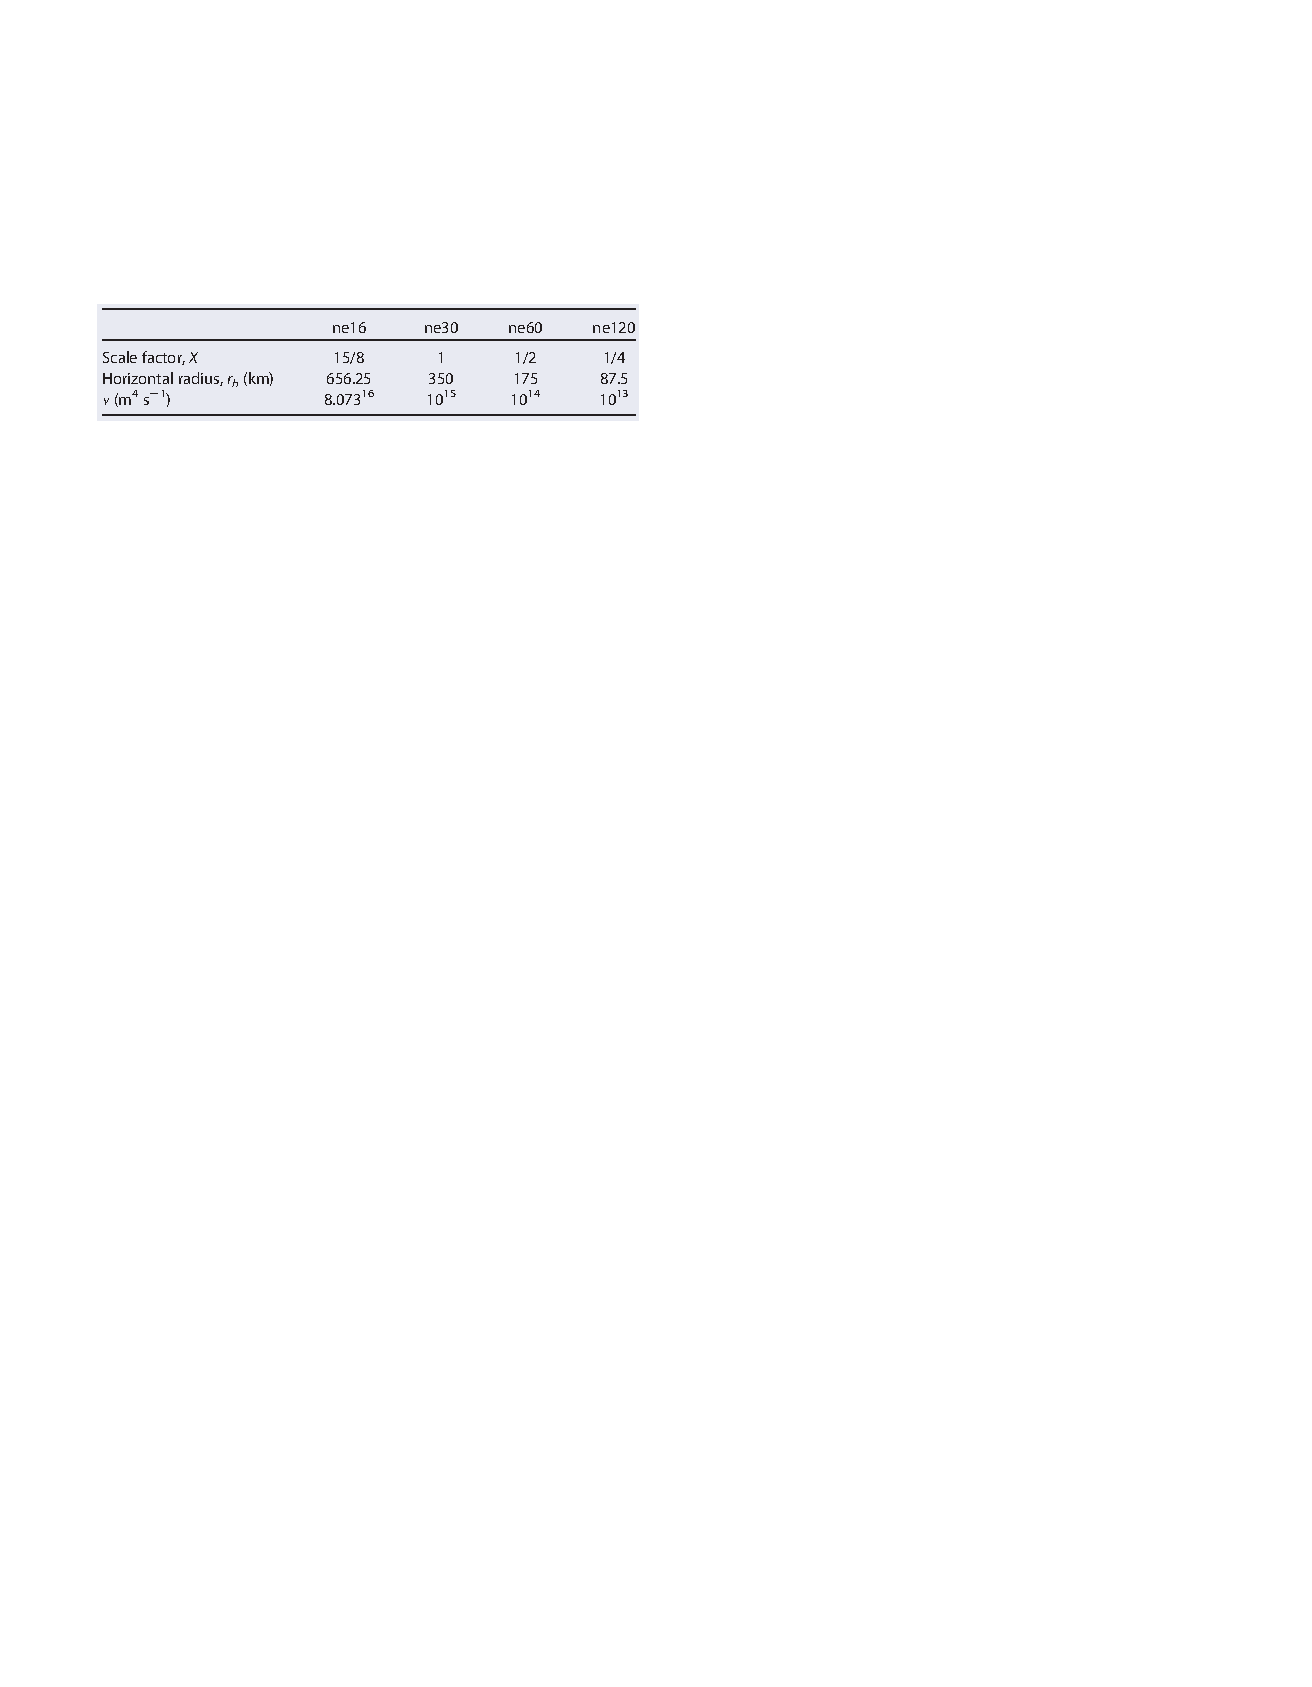
\includegraphics[width=25pc,angle=0]{chapter3/table2.pdf}\\
\end{center}
\caption{Scale factors ($X$) used to scale Earth’s planetary radius to match the horizontal resolution of other grids (header), as well as the horizontal bubble radius ($r_h$) and hyper-viscosity coefficients ($\nu$), for each equivalent resolution.}
\label{tbl:table3-2}
\end{table}

Through fixing the initial conditions, and multiplying the planetary radius, $a$, by the scale factor $X$, $r_h$ is varied by the same factor as $\Delta x$. In the style of \cite{RM2016GRL}, the scale factors are defined as the coefficients required to scale the Earth’s planetary radius to match the horizontal resolutions used in the aqua-planet simulations (Table~\ref{tbl:table3-2}). We set the horizontal diameter of the moist bubbles to about seven times the grid spacing (specifically, we set $r_h = 350$ km at Earth’s planetary radius) and a vertical diameter of 4 km ($r_z = 2$ km), which is comparable to the horizontal and vertical scales of diabatic forcing in the aqua-planet simulations (Figure~\ref{fig:figure3-1}). 

Two additional important parameters are the vertical location of the bubble ($z_c$) and the magnitude ($\Delta \theta$). A smaller $z_c$ or larger $\Delta \theta$ both lead to increased available potential energy, and potentially greater vertical motion. Figure~\ref{fig:figure3-1} indicates that large-magnitude stratiform tendencies are common in the Tropical upper-troposphere at all resolutions. The diabatic forcing depicted in Figure~\ref{fig:figure3-1} correspond to potential temperature perturbations on the order of 1 K. Despite the prevalence of the upper-troposphere structures, we opt for a more extreme initial condition, one that is less common in the simulations, to encourage non-linearity that could potentially break the scaling of equation~\ref{eq:eq3-3}. Plots of the initial conditions for the moist experiments are provided in Figure~\ref{fig:figure3-2}, depicting a bubble with a magnitude of 3K, a vertical extent much less than the depth of the troposphere, and located just above the nominal boundary layer. Table~\ref{tbl:table3-3} provides a list of all parameters used to generate the initial conditions for the experiments.

\begin{table}
\begin{center}
\noindent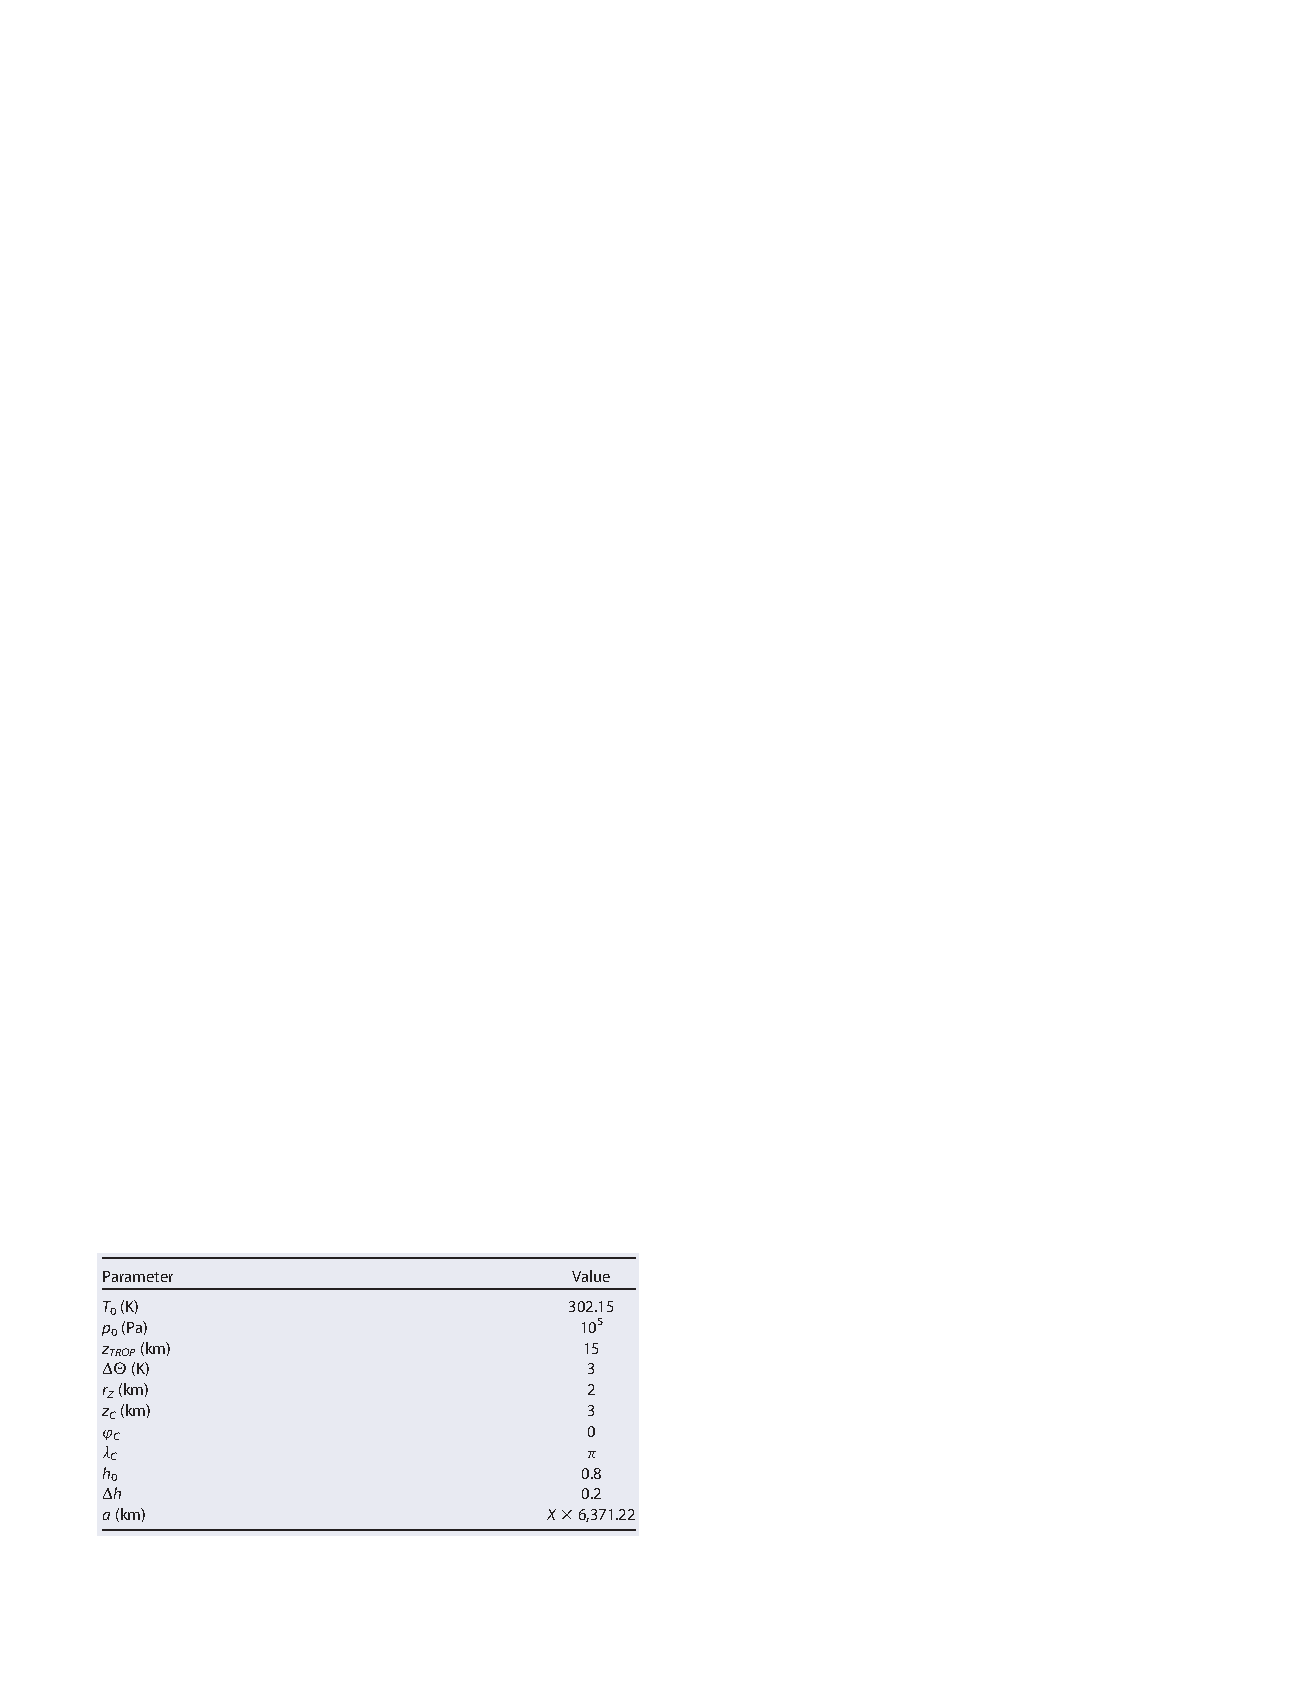
\includegraphics[width=20pc,angle=0]{chapter3/table3.pdf}\\
\end{center}
\caption{Parameters used in generating the initial conditions for the dry and moist experiments. $X$ is the scale factor, provided in Table~\ref{tbl:table3-2}.}
\label{tbl:table3-3}
\end{table}

\begin{figure}
\begin{center}
\noindent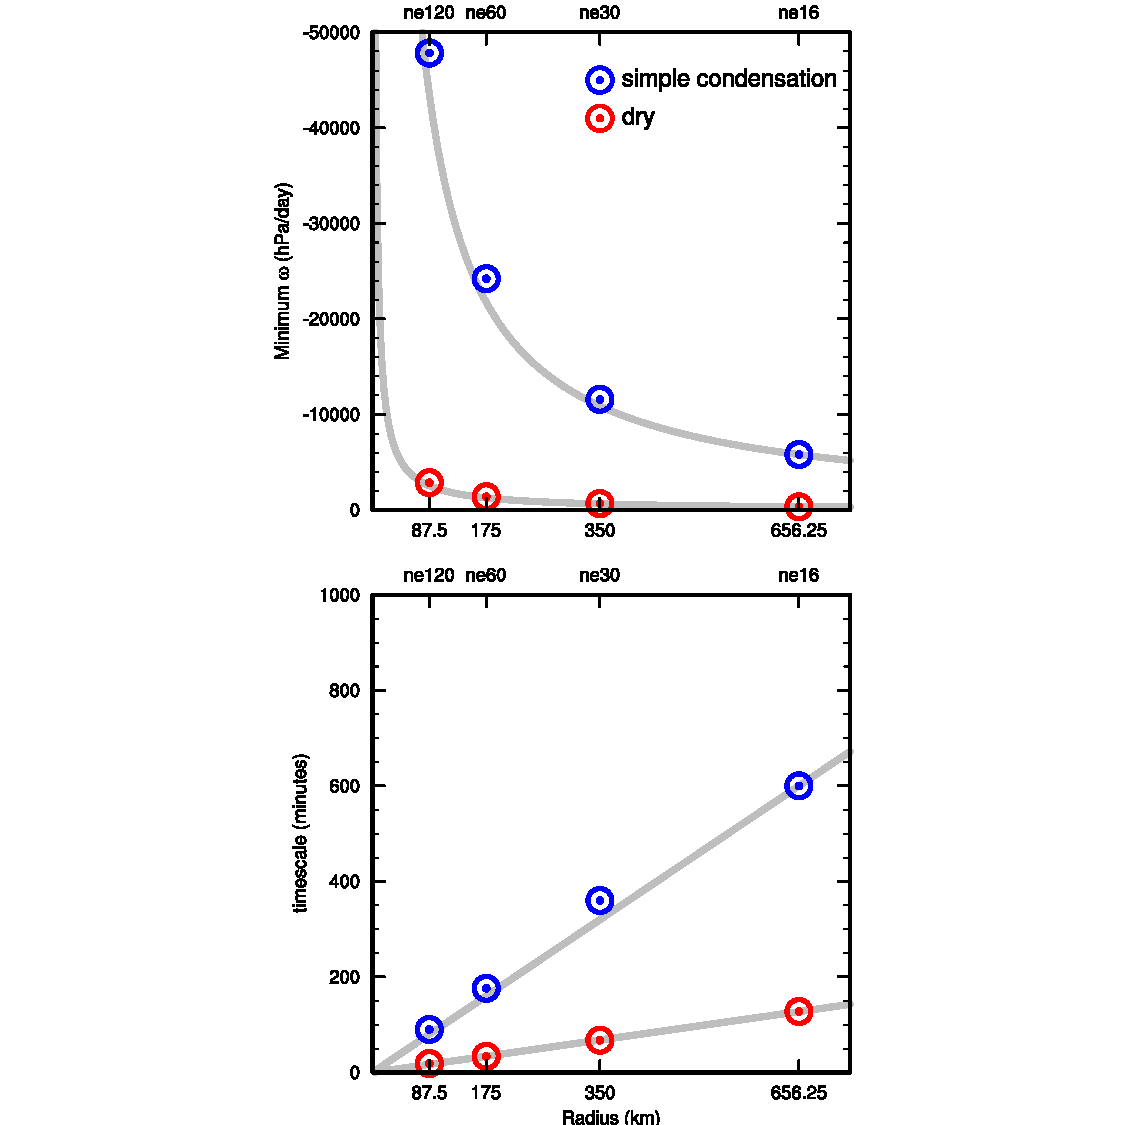
\includegraphics[width=20pc,angle=0]{chapter3/Figure3_crop.pdf}\\
\end{center}
\caption{Results of the experiments using the simple condensation scheme and an equivalent configuration without moisture (`dry’). (Top) minimum vertical pressure velocity, $\omega$, over the duration of each experiment as a function of bubble radius (Bottom) the model time associated with the minimum in $\omega$ as a function of bubble radius. The top axis indicates the equivalent horizontal resolution of the grid used to simulate a particular bubble radius. Grey lines represent the scaling of equation~\ref{eq:eq3-3}, scaled by the lowest resolution (ne16) solution.}
\label{fig:figure3-3}
\end{figure}

\subsection{Results}
\subsubsection{CAM-SE without moisture}
Before embarking on an analysis of the moist experiments, we first consider the behavior of an experiment which contains no moist processes. The red markers in Figure~\ref{fig:figure3-3} are the results of a dry experiment, i.e. the initial conditions are those of Figure~\ref{fig:figure3-2}, but with no specific humidity. The blue markers are the results from a moist experiment, and are discussed in the next section. Results are displayed as the minimum vertical pressure velocity, $\omega$, over the duration of each experiment as a function of $r_h$. The $1/r_h$scaling implied by equation~\ref{eq:eq3-3} is overlain as a grey line, scaled by the lowest resolution simulation. The analytical scaling and the model experiments agree to a remarkable extent, indicating that the model dynamics are adequately described by the simple scale analysis of equation~\ref{eq:eq3-3} for the case of a dry, rising bubble.

\begin{figure}
\begin{center}
\noindent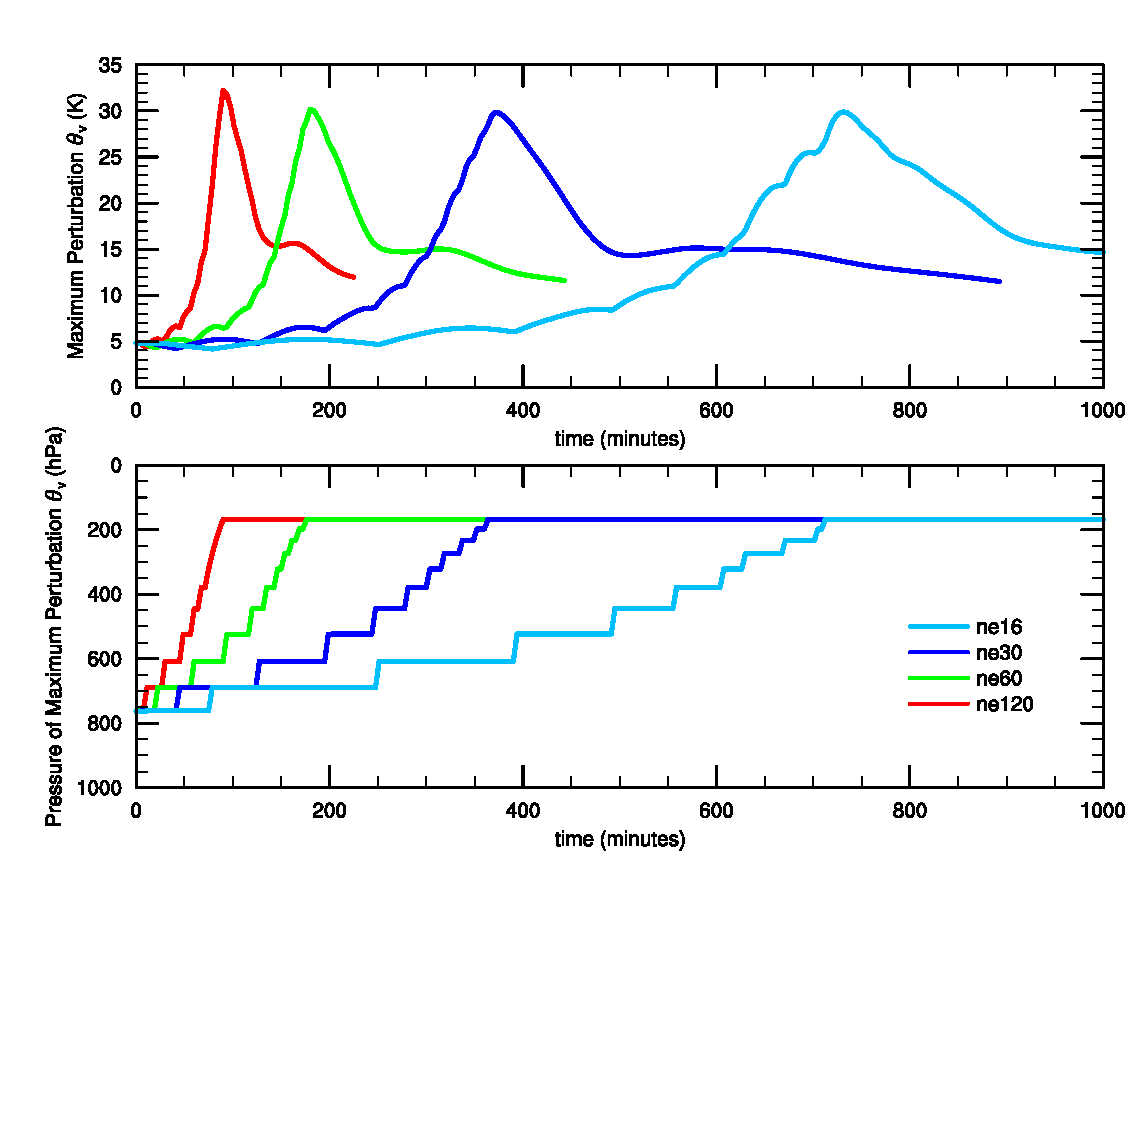
\includegraphics[width=25pc,angle=0]{chapter3/Figure4_crop.pdf}\\
\end{center}
\caption{Time series of the maximum perturbation $\theta_v$ (top) and the pressure associated with this maximum (bottom) in the moist experiment using the simple condensation scheme.}
\label{fig:figure3-4}
\end{figure}

\subsubsection{CAM-SE coupled to the Simple Condensation Scheme}
Figure~\ref{fig:figure3-3} also shows the results of the moist experiment with CAM-SE coupled to the simple condensation scheme. The simple moist experiments obey the linear scaling of equation~\ref{eq:eq3-3}, despite the inclusion of moist processes. This is not a trivial result since the analytical scaling (equation~\ref{eq:eq3-3}) was derived without any treatment of moist processes. Moisture does however amplify the vertical motion by about an order of magnitude compared to the dry case, with $\omega$ approaching $-50 \times 10^3$ hPa day$^{-1}$, or about 20 m s$^{-1}$. Whereas the dry bubbles are unable to reach the tropopause, the moist bubbles maintain their structures all the way to the tropopause, owing to a much larger reservoir of available potential energy.
 
The minimum vertical pressure velocities in the moist tests are attained once the moist bubble reaches the tropopause. This can be determined by comparing the timescales in Figure~\ref{fig:figure3-3} to the time evolution of the bubble pressure (Figure~\ref{fig:figure3-4}). Figure~\ref{fig:figure3-4} also shows that the minimum in $\omega$ are associated with a maximum virtual potential temperature ($\theta_v$) perturbation, defined as the difference in $\theta_v$ from the initial reference state. The maximum $\theta_v$ perturbation is approximately invariant to bubble radius, indicating the difference in $\omega$ across resolutions are almost entirely a result of the $1/r_h$ scaling, as opposed to a change in available potential energy ($\sqrt{B_0 H}$ in equation~\ref{eq:eq3-3}). The scaling fits the moist experiments well since the horizontal scale of the moist bubbles do not change significantly as they ascend to their level of neutral buoyancy (i.e., the tropopause).

\begin{figure}
\begin{center}
\noindent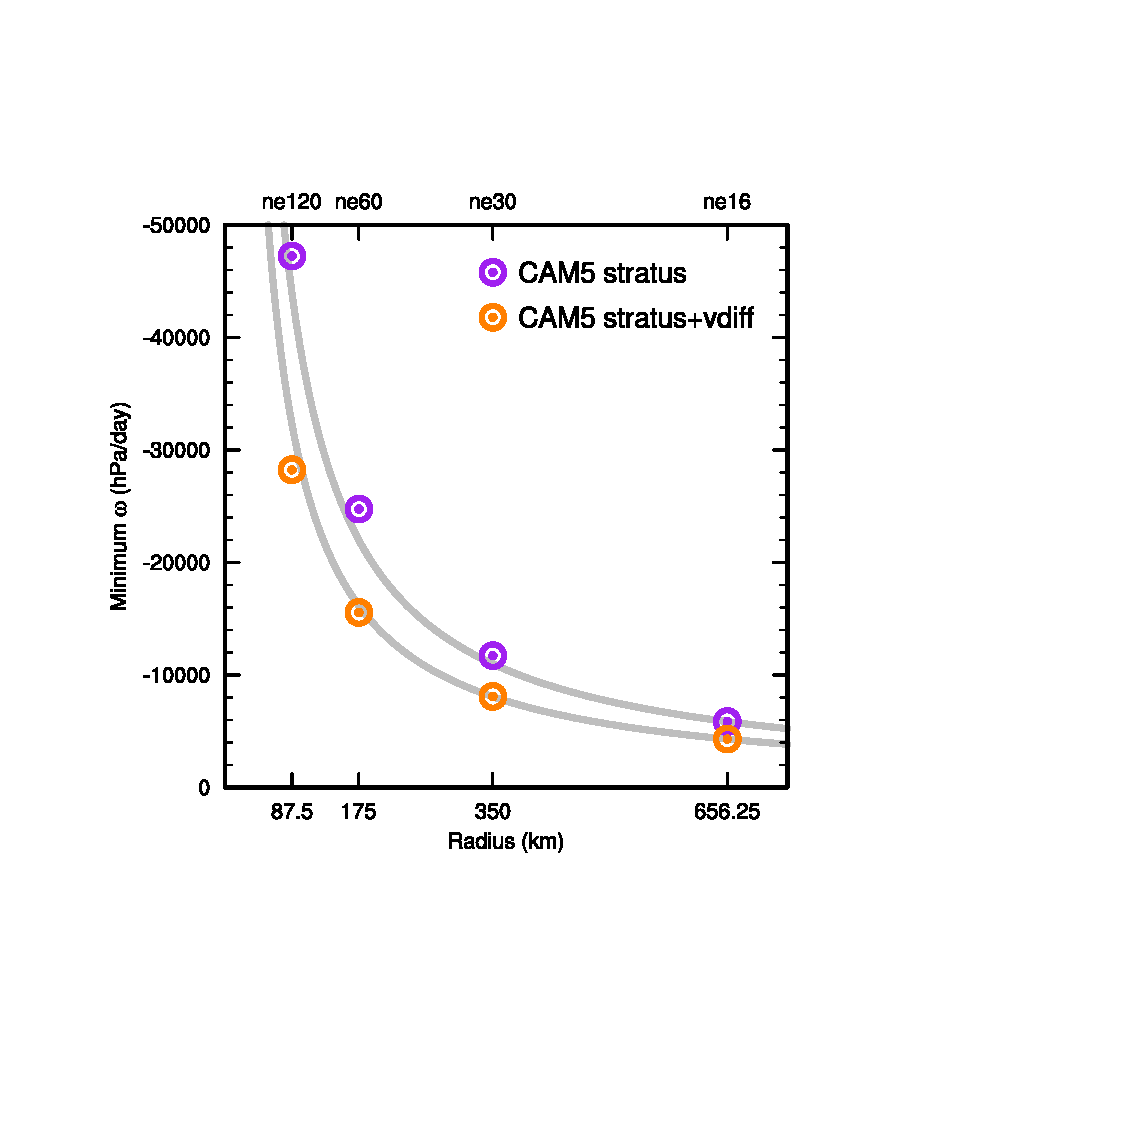
\includegraphics[width=20pc,angle=0]{chapter3/Figure5_crop.pdf}\\
\end{center}
\caption{As in Figure~\ref{fig:figure3-3}, but for the moist experiments using the CAM5 stratiform scheme (‘stratus’) and the CAM5 stratiform scheme coupled with the CAM5 vertical diffusion routine (‘stratus$+$vdiff’).}
\label{fig:figure3-5}
\end{figure}

\subsubsection{CAM-SE coupled to CAM5 Moist Physics}
The moist experiments are repeated using the more complex physics modules contained in the CAM5 physics package. Despite the increased complexity of the CAM5 stratiform cloud scheme (labeled as “stratus”) compared with the simple condensation scheme, the magnitudes of $\omega$ across the four different resolutions are nearly identical (Figures \ref{fig:figure3-5} and \ref{fig:figure3-3}). The inclusion of vertical dissipation (labeled as “stratus+vdiff”) reduces the magnitude of $\omega$ by about 40\%, but preserves the $1/r_h$ scaling (Figure~\ref{fig:figure3-5}). This is achieved through reducing the magnitude of the Archimedean buoyancy by local downgradient vertical mixing, but the scheme is unable to affect its horizontal scale. We conclude that the incorporation of moist processes, short of a convection scheme, maintains a physical response analogous to the physics of the dry system (equation~\ref{eq:eq3-3}).

\subsubsection{Sensitivity to physics time-step}
\paragraph{CAM-SE} ~\\
In all the moist experiments discussed so far, the physics time-step is set to 225 s. In practice, a longer physics time-step is used to minimize the computational overhead associated with the physics routines. For example, the default physics time-step in the ne30 configuration is 1800 s, and the experiments analyzed in \cite{HR2017JCLIM} use a physics time-step of 600 s. To explore the implications of using longer physics time-steps, the moist experiments are ran using physics time-steps of 450 s, 900 s and 1800 s. These experiments are performed using the simple condensation scheme and the CAM5 stratiform scheme.

\begin{figure}
\begin{center}
\noindent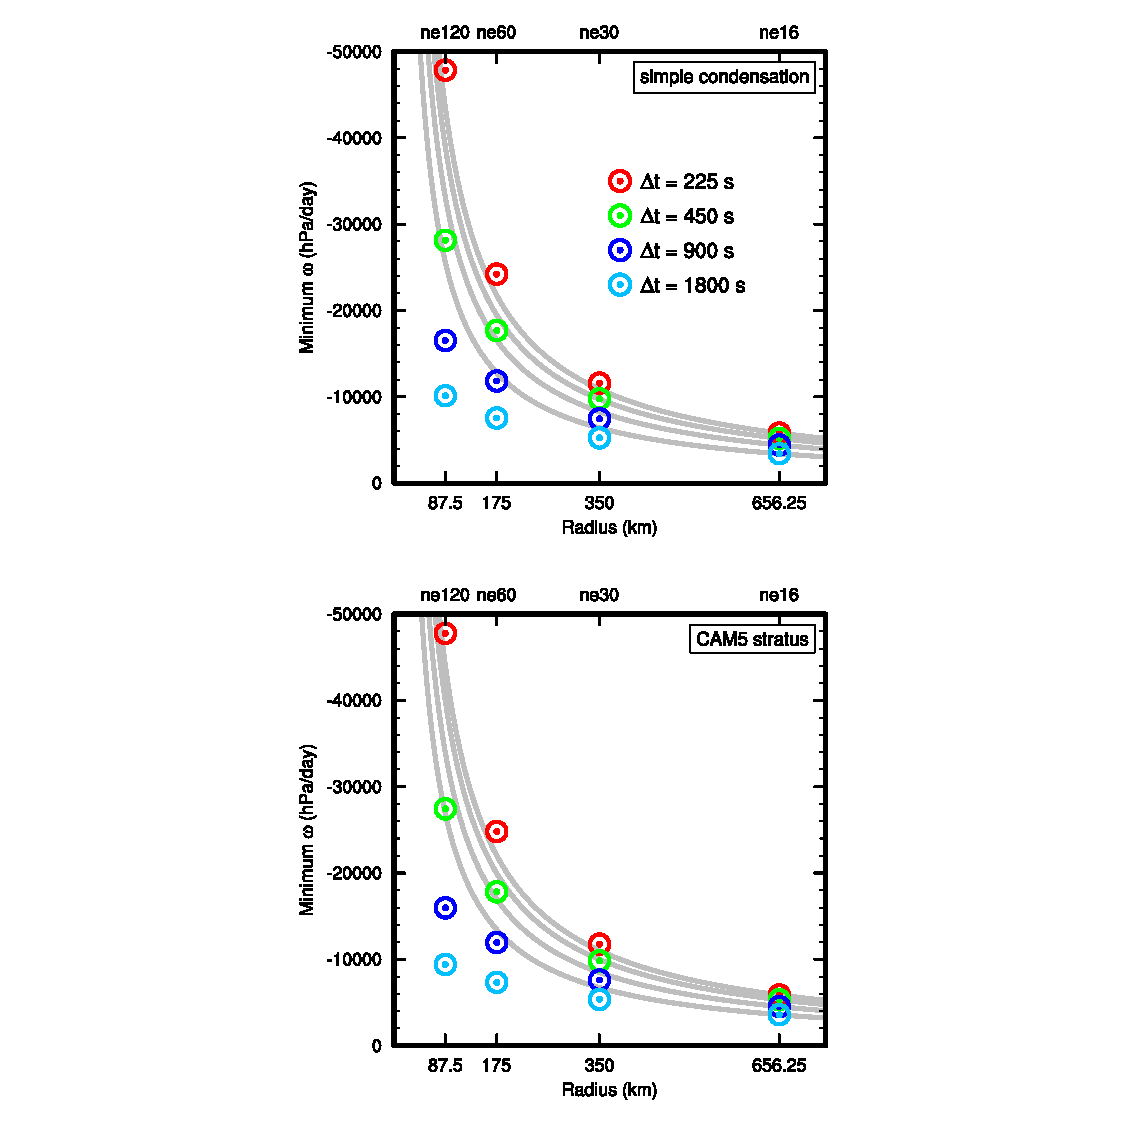
\includegraphics[width=20pc,angle=0]{chapter3/Figure6_crop.pdf}\\
\end{center}
\caption{As in Figure~\ref{fig:figure3-5}, but for the physics time-step sensitivity experiments using the simple condensation scheme (top) and the CAM5 stratiform scheme (bottom).}
\label{fig:figure3-6}
\end{figure}

The results of the physics time-step experiments for the two different condensation routines are shown in Figure~\ref{fig:figure3-6}. The time-step sensitivity using only the CAM5 stratus parameterization is almost identical to the time-step sensitivity of the simple condensation scheme (Figure~\ref{fig:figure3-6}). For a physics time-step of 450 s, the simulations begin to depart from the $1/r_h$ scaling observed in the 225 s experiments, damping the vertical motion at smaller $r_h$. At longer physics time-steps, the departure from $1/r_h$ scaling is even greater.

\paragraph{CAM-FV} ~\\
The time-step sensitivity experiment using the CAM5 stratiform routine has been repeated using the CAM-FV dynamical core (Figure~\ref{fig:figure3-7}). The magnitude of $\omega$ in CAM-FV is about 50\% less than in CAM-SE, at all resolutions (Figures \ref{fig:figure3-6} and \ref{fig:figure3-7}). This is consistent with simulations of tropical cyclones using these two dynamical cores – CAM-SE tends to have stronger storms as compared with CAM-FV \citep{RJ2012JAMES,RETAL2012ASL,RETAL2015JAS}. The qualitative behavior of the response to resolution and time-stepping is however, similar to CAM-SE – $\omega$ generally follow the scaling at small physics time-steps, but depart from the scaling at longer physics time-steps (Figure~\ref{fig:figure3-7}). Note that the $\omega$ field in the $2^{\circ}$ runs do not follow the scaling (not shown). To observe the scaling in CAM-FV at small physics time-steps, one must scale to a resolution other than $2^{\circ}$ (Figure~\ref{fig:figure3-7}).

\begin{figure}
\begin{center}
\noindent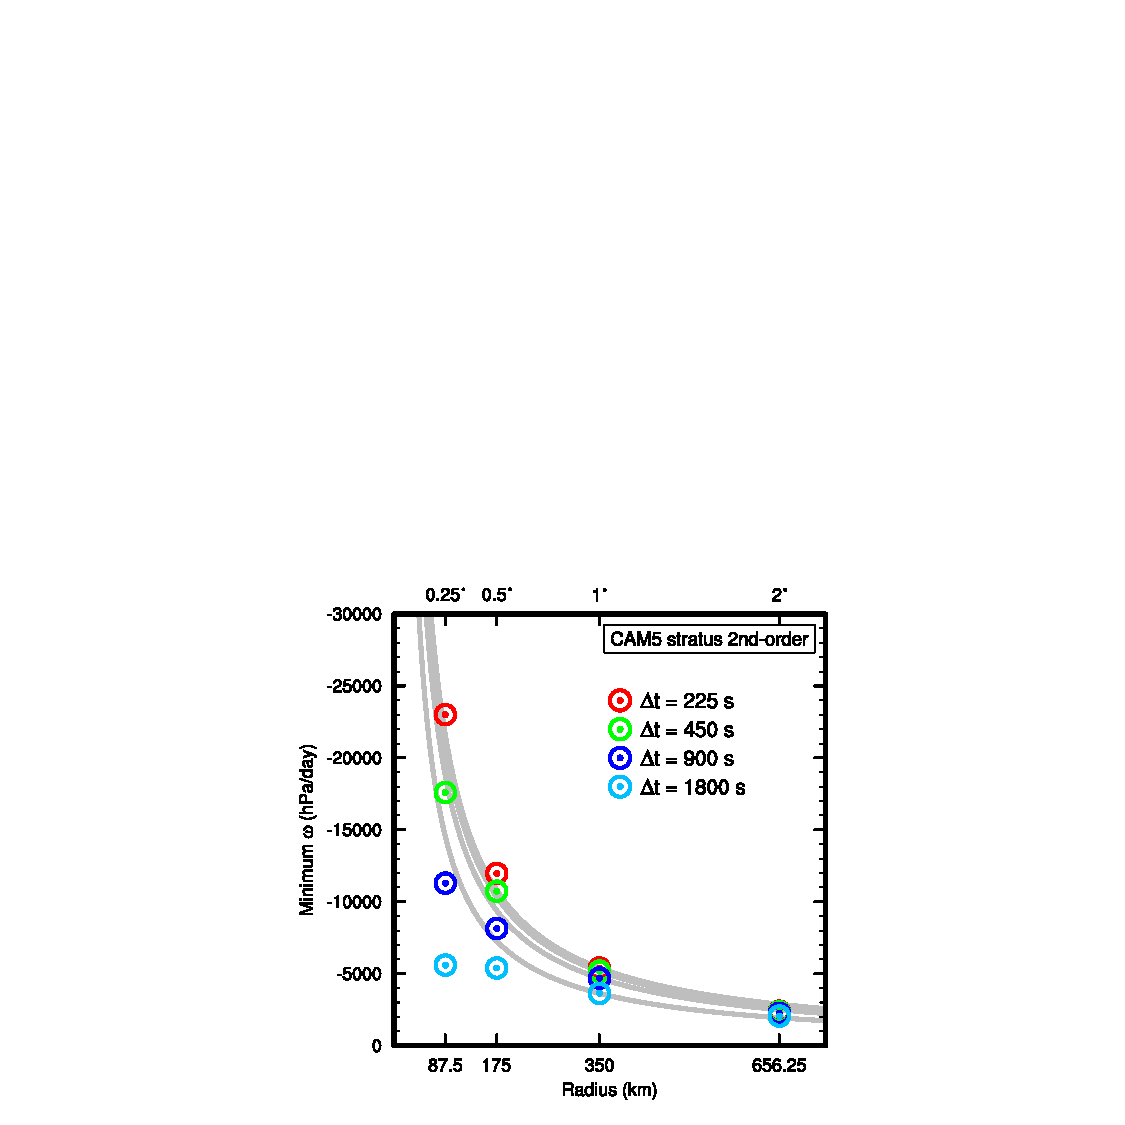
\includegraphics[width=20pc,angle=0]{chapter3/Figure7_crop.pdf}\\
\end{center}
\caption{As in Figure~\ref{fig:figure3-6}, but using the CAM-FV with second-order divergence damping. Note the analytical scaling (grey lines) have been scaled to the $1^{\circ}$ simulation in this plot, and the y-axis range in smaller, compared with Figure~\ref{fig:figure3-6}.}
\label{fig:figure3-7}
\end{figure}

The time-step sensitivity experiments in CAM-FV are repeated using the fourth-order divergence dampening operator, resulting in slightly lower magnitude vertical pressure velocities, but otherwise the experiment depicts a very similar sensitivity to physics time-step as the second order divergence damping simulation (not shown). The minimum $\omega$ in the simulation using the 225 s physics time-step and a $0.25^{\circ}$ grid, is -20179.8 hPa/day, compared to -23008.7 hPa/day with the second-order divergence damping. This result is intuitive – the higher the order of the divergence damping operator, the more effectively it damps near grid-scale features \citep{WJRL2010MWR}, such as the $\sim 7 \Delta x$ moist bubbles.

The fourth-order, internally computed divergence damping coefficient was found to be about twice as large as that used by CAM-SE. An additional simulation using the $0.25^{\circ}$ grid and 225 s time-step, in which the fourth-order divergence damping coefficient is lowered by an order of magnitude, results in an increase in the magnitude of $\omega$ by from -20179.8 hPa/day to -24689.7 hPa/day. The time-series of the minimum vertical pressure velocities in this simulation is compared to the equivalent CAM-SE simulation, in Figure~\ref{fig:figure3-8}, along with the CAM-FV simulation using the default fourth order divergence damping coefficient. While the larger divergence-damping coefficient used in CAM-FV may explain a portion of the differences between the CAM-SE and CAM-FV solutions, it does not explain most of the differences between the two solutions (Figure~\ref{fig:figure3-8}). The lower magnitude $\omega$ in CAM-FV may be a result of the diffusive nature of finite-volume numerics and/or limiters in the CAM-FV dynamical core \citep{LR1997QJR}, but could also be related to unphysical numerical aspects of the continuous Galerkin method, potentially resulting in artificially large magnitude  in CAM-SE. Further testing is required to provide conclusive evidence of the design aspects leading to the differences in solutions between these two dynamical cores.

\begin{figure}
\begin{center}
\noindent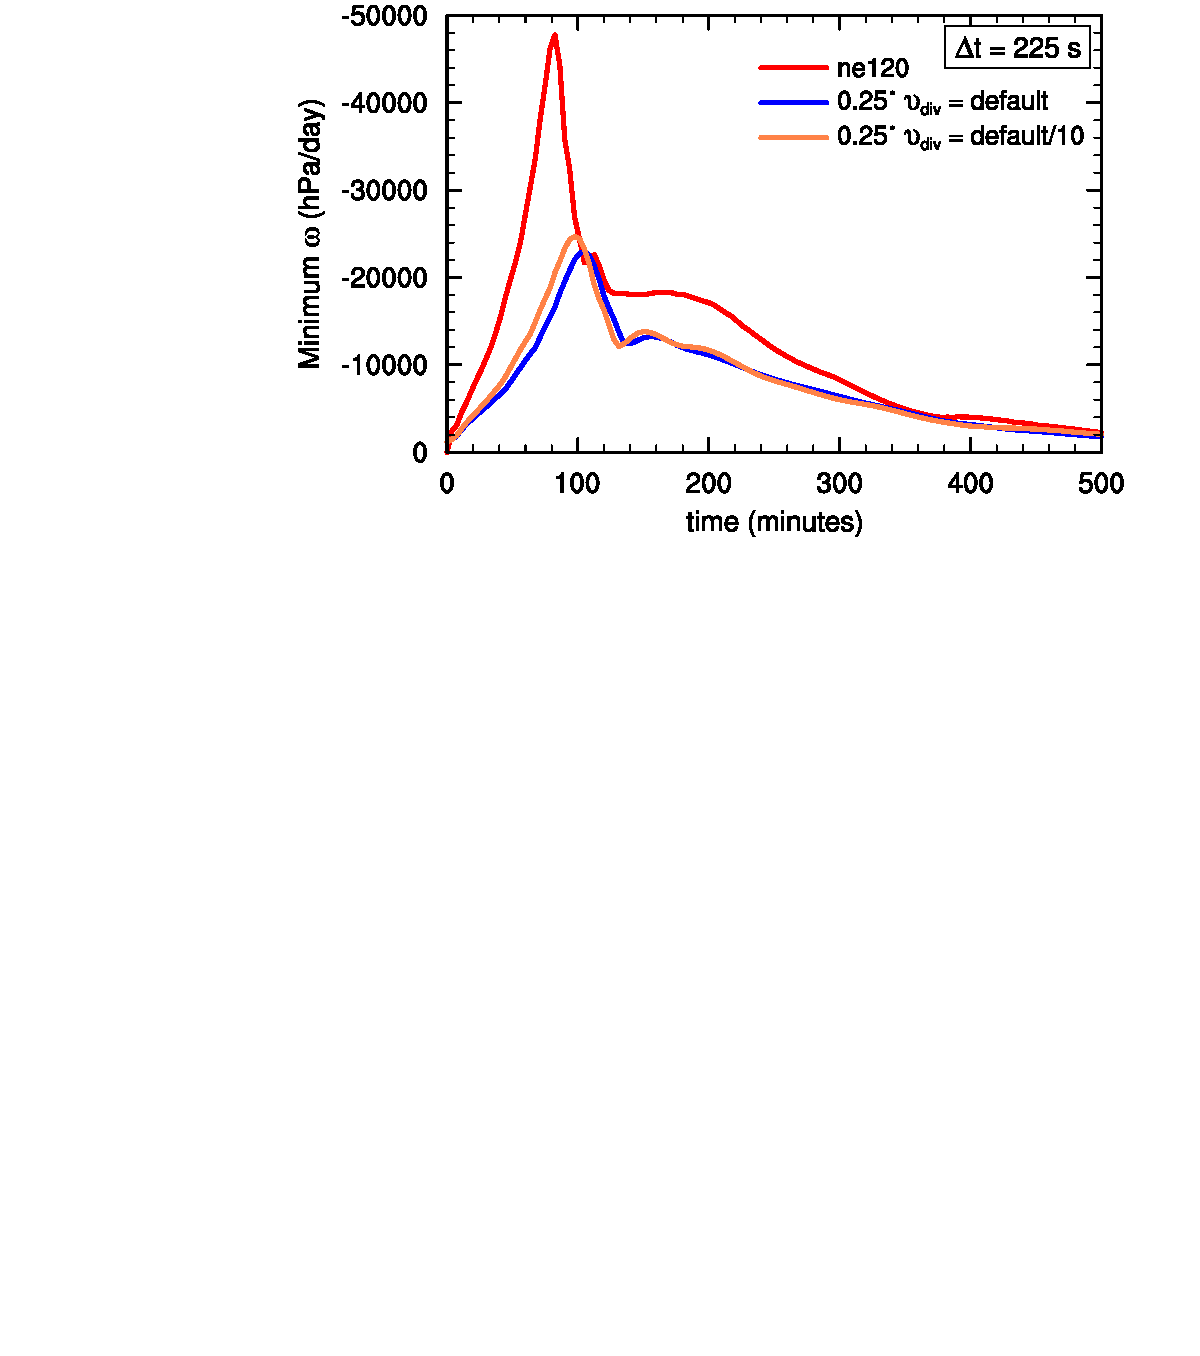
\includegraphics[width=25pc,angle=0]{chapter3/Figure8_crop.pdf}\\
\end{center}
\caption{Time-series of the minimum in $\omega$ for three different moist bubble simulations using the CAM5 stratiform scheme and a physics time-step of 225 s, at the highest grid resolution. The CAM-SE run is labeled `ne120’, while a pair of CAM-FV simulations using the fourth-order divergence damping are depicted, one using the default divergence damping coefficient, and another simulation with the coefficient reduced by an order of magnitude.}
\label{fig:figure3-8}
\end{figure}

\paragraph{Sensitivity to viscosity} ~\\
Through reducing the specific humidity hyper-viscosity coefficient in CAM-SE by an order of magnitude, the vertical velocity scaling is nearly recovered using a 450 s time-step (Supplementary Figure~\ref{fig:sfigure3-2}). Through individually reducing the hyper-viscosity coefficients on the other state variables (temperature, pressure thickness, non-divergent and divergent winds), the solutions either did not improve the scaling as effectively as the coefficient for specific humidity, or the model failed (note that the specific value of the coefficients are chosen by model developers, in part, for numerical stability). For example, model failure was common when reducing the divergence damping coefficient. In the simulations that did not crash, reducing the divergence damping coefficient by an order of magnitude lead to an increase in the magnitude of the vertical motion at all resolutions, but it’s effect on the scaling is ambiguous, and not as clear as the experiment in which specific humidity coefficient is reduced (Supplementary Figure~\ref{fig:sfigure3-2}).

\begin{figure}
\begin{center}
\noindent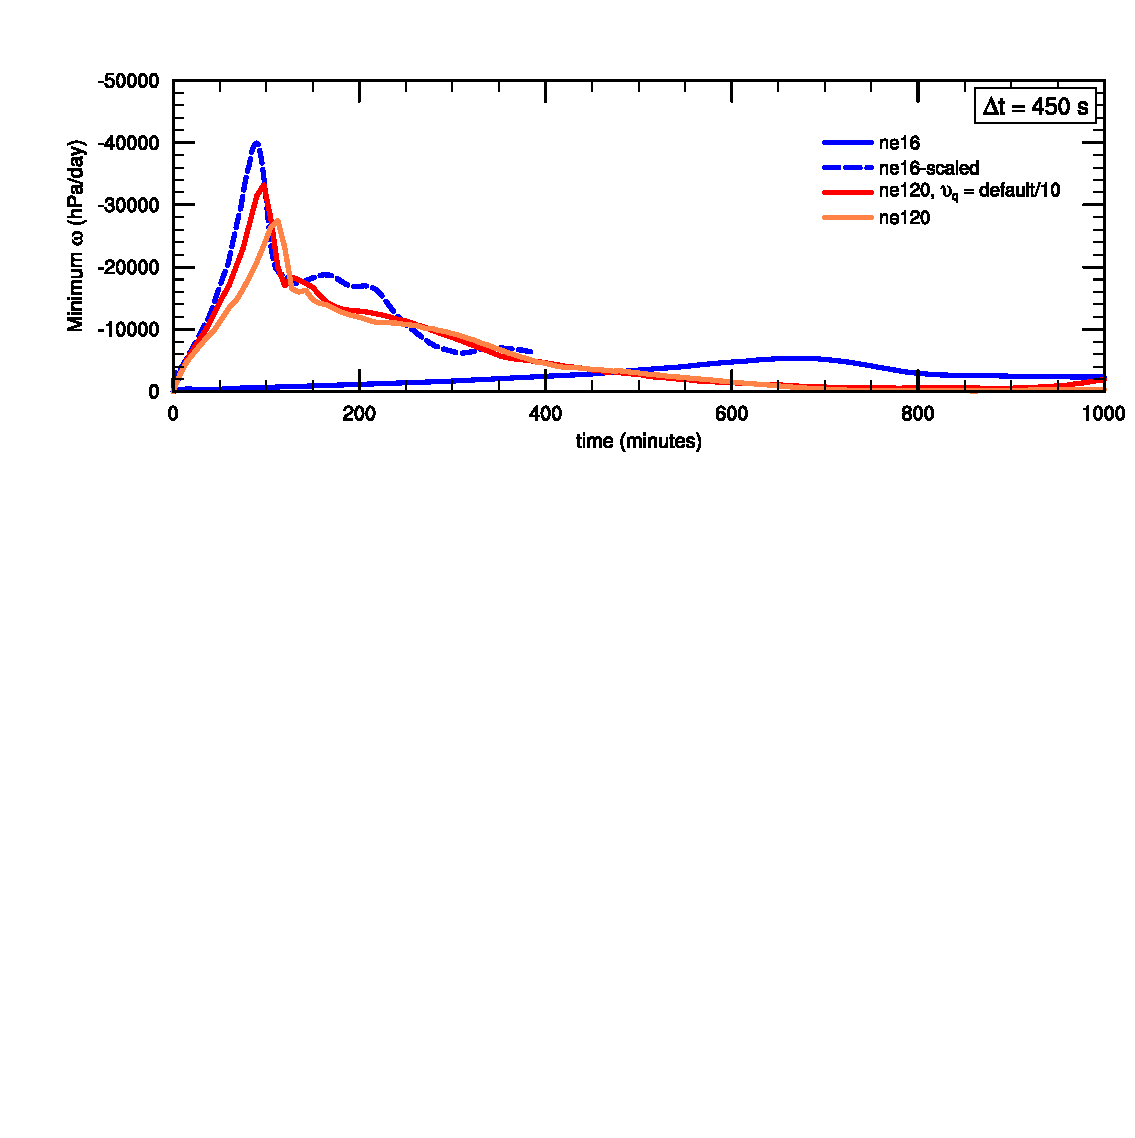
\includegraphics[width=35pc,angle=0]{chapter3/Figure9_crop.pdf}\\
\end{center}
\caption{Time-series of the minimum $\omega$ in three different CAM-SE moist bubble simulations using the CAM5 stratiform scheme and a physics time-step of 450 s. The dashed line shows the results of an ne16 simulation scaled to the ne120 resolution using equation~\ref{eq:eq3-3}. The orange line denotes the ne120 resolution simulation, while the red line is an ne120 simulation with the specific humidity hyper-viscosity coefficient reduced by an order of magnitude.}
\label{fig:figure3-9}
\end{figure}

Figure~\ref{fig:figure3-9} depicts the time dependence of the simulation in which the specific humidity hyper-viscosity coefficient is reduced by an order of magnitude. The results are presented as a time-series of the minimum $\omega$ in the highest resolution simulation, using a physics time-step of 450 s. The target solution, i.e., the solution found by scaling the lowest resolution simulation to the highest resolution using equation~\ref{eq:eq3-3}, as well as the highest resolution simulation using the default hyper-viscosity coefficients, are also shown in Figure~\ref{fig:figure3-9}. Through reducing the specific humidity coefficient, the ne120 solution approaches, but still underestimate, the target solution (Figure~\ref{fig:figure3-9}).

\subsection{Discussion}
The idealized experiments are evidence that the scaling of equation~\ref{eq:eq3-3} is maintained in a moist physics configuration, basically a two-component idealization of an AGCM containing only a dynamical core and large-scale condensation scheme, across multiple resolutions. Extending our results to the vertical velocity scaling observed in more complex configurations, such as aqua-planet experiments (e.g., Figure~\ref{fig:figure3-1}), may be a stretch. The CAM5 moist physics package contains shallow \citep{PB2009JC} and deep \citep{ZM1995AO,RR2008JC,NRJ2008JC} convection schemes. The large, predominantly stratiform thermals occurring only within the upper-troposphere in Figure~\ref{fig:figure3-1}, and the associated re-evaporation of falling condensate within the lower troposphere, are related to the deep convection scheme, and are designed to represent the effects of anvil cloud top formation in a deep convective system \citep{CAM5,PETAL2014JCLIM}. 

The source of moisture for the anvil tops in the model is primarily through detrainment of parameterized deep convective plumes, although moisture transport by the resolved dynamics and/or parameterized deep convective mass fluxes may be important as well. The anvil tops are confined to within the upper-troposphere because detrainment of the plume air is only permitted above the vertical level pertaining to the minimum in moist static energy \citep{ZM1995AO}. The deep convection scheme is designed to remove unstable air originating in the planetary boundary layer through vertical redistribution, severely limiting its ability to reduce the unstable conditions created through anvil cloud top formation. Therefore, to understand the model response to the rather popular anvil cloud tops (Figure~\ref{fig:figure3-1}), the reduced stratiform-dynamical core system may not be a terrible approximation. The initial conditions used in the idealized moist bubble experiments contain unstable conditions only above the planetary boundary layer, and a separate run using the complete CAM5 moist physics package confirms that the deep convection scheme is not triggered by the initial conditions (not shown).

It is not common for climate models to be ran using a physics time-step as small as 225 s, potentially explaining why the aqua-planet simulations of \cite{HR2017JCLIM} utilizing a 600 s physics time-step, or those discussed in the introduction using an 1800 s time-step (Figure~\ref{fig:figure3-10}, dashed lines), do not follow the vertical velocity scaling of equation~\ref{eq:eq3-3} across resolutions. To test this idea, four additional CAM-SE aqua-planet experiments are run, utilizing two different resolutions, ne30 and ne120. All four simulations are as described in the introduction, and are run for one year. The dynamics time-step was fixed between the two resolutions, set to 75 s, and each resolution is simulated twice using physics time-steps of 1800 s and then 225 s. The results of these four simulations are depicted in Figure~\ref{fig:figure3-10} as a probability density distribution of the negative $\omega$ at all vertical levels between $10^{\circ}$N and $10^{\circ}$S, computed from 6-hourly output over the final 11 months of the integration. The ne30 solutions are expressed as the ne30 probability density distribution scaled to the ne120 resolution following \cite{PG2006JAS},
\begin{equation}
P(\omega_1) = \alpha P(\omega_0 / \alpha), \label{eq:eq3-8}
\end{equation}
where $P(\omega)$ is the probability density distribution of the vertical pressure velocity, the subscripts refer to two different resolutions, $\Delta x_0$ and $\Delta x_1$, and $\alpha$ is the ratio of the velocity scale at $\Delta x_0$ to the velocity scale at $\Delta x_1$. Assuming the characteristic buoyancy of parcels in a simulation is unchanged between two resolutions, then through assuming $D \propto \Delta x$, $\alpha = \Delta x_1 / \Delta x_0$ from equation~\ref{eq:eq3-3}.

\begin{figure}
\begin{center}
\noindent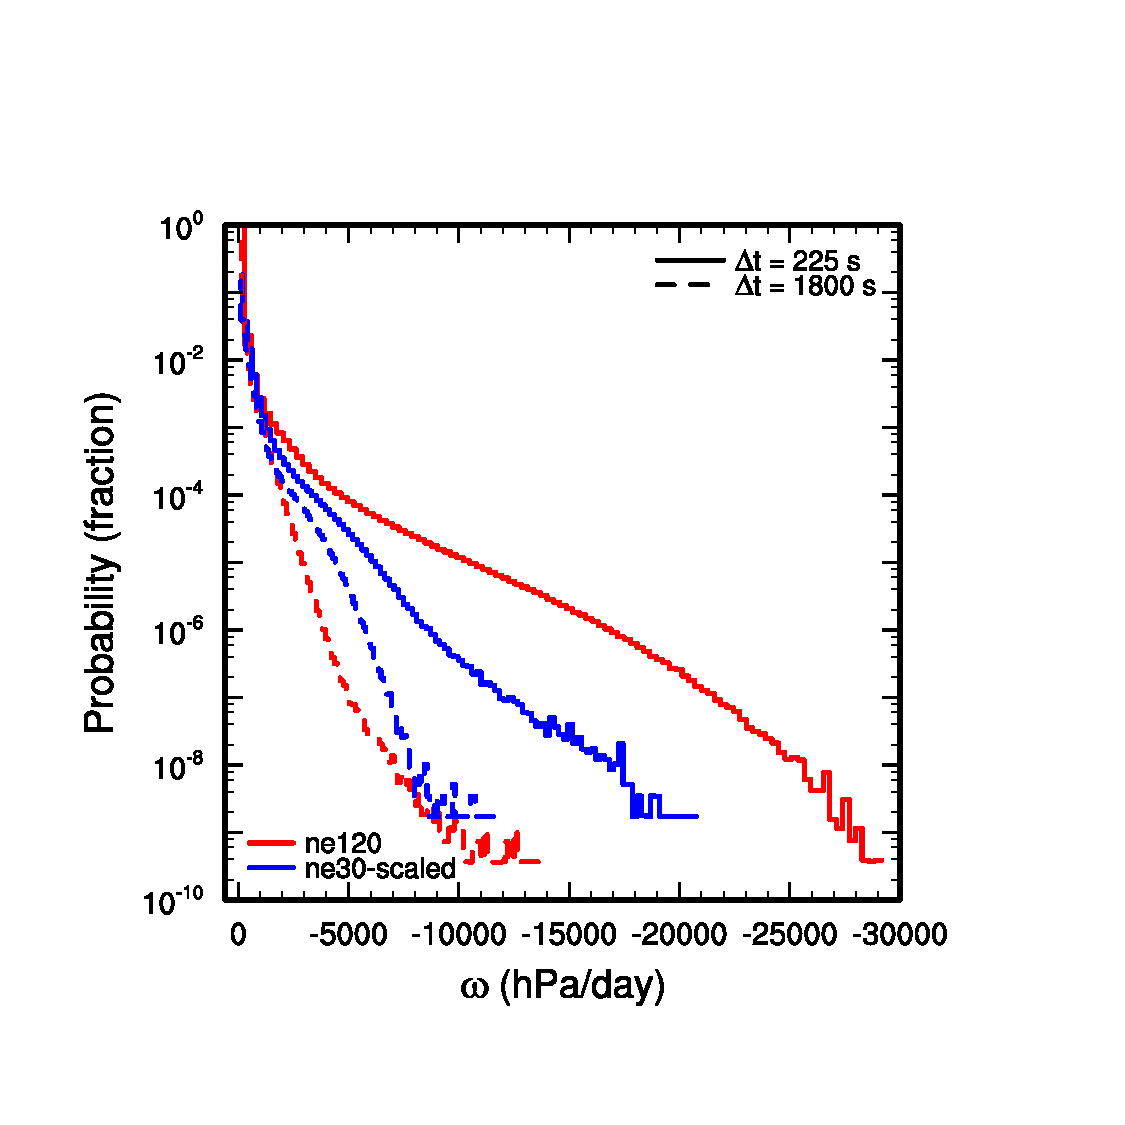
\includegraphics[width=20pc,angle=0]{chapter3/Figure10_crop.pdf}\\
\end{center}
\caption{Probability density distribution of negative  at all levels, and between $10{\circ}$N and $10^{\circ}$S, for four different aqua-planet simulations. An ne30 and ne120 simulation are depicted with colors, and the physics time-step used in the simulations are shown in different line styles. The ne30 solutions are expressed as ne30 solutions scaled to the ne120 resolution, as described in the text.}
\label{fig:figure3-10}
\end{figure}

Using an 1800 s physics time-step results in the usual scenario, with the scaled ne30 solutions generally over-predicting the occurrence of the ne120 upward  $\omega$ (Figure~\ref{fig:figure3-10}), although the mismatch is not as severe as in \cite{HR2017JCLIM}. This result is consistent with the moist bubble experiments - the over-prediction of vertical motion occurs using the 1800 s physics time-step (Figure~\ref{fig:figure3-6}). In contrast, with the 225 s physics time-step, the scaled ne30 solutions now under-predict the occurrence of large-magnitude vertical motion at high resolution (Figure~\ref{fig:figure3-10}), which does not occur in the moist bubble experiments (Figure~\ref{fig:figure3-6}). Reducing the physics time-step leads to larger magnitude vertical motions at both resolutions, which is apparent from the longer tails of the distributions (Figure~\ref{fig:figure3-10}). While the 225 s time-step simulations does not necessarily improve the ability of the scaling to explain the resolution sensitivity, the aqua-planet experiments are nonetheless consistent with idealized moist bubble experiments – the magnitude of the vertical motion is dampened through the use of longer physics time-steps, and more-so at higher resolution. 

One should bear in mind that comparing the relatively coarse time-sampling of the instantaneous $\omega$ in the aqua-planets (6-hourly) to the scaling derived from the high-frequency output (from 225 s to 1800 s) of the minimum $\omega$ in the moist bubble tests, may be reason alone for the observed difference in scaling between the two configurations. While the authors feel that the sampling bias is mitigated to some extent through the use of a large sample size to compute the aqua-planets statistics, concerns regarding dataset inconsistency have not been thoroughly explored.

The authors speculate that the mismatch between scaled and the actual solutions at short physics time-steps in the aqua-planets are due to a non-negligible change in thermodynamic properties of thermals across resolutions. One example leading to such a change is the occurrence of grid-point storms at high resolution and small physics time-steps, reported in \cite{W2013QJRMS}. Compared with the ne30 simulation, the response of the ne120 simulation to the shorter physics time-step leads to a proportionally larger increase in the magnitude of $\omega$ (Figure~\ref{fig:figure3-10}). The probability density distributions presented in \cite{W2013QJRMS} suggests that extreme values of $\omega$ in the tails of the distribution, such as occur in the ne120, 225 s time-step simulation (Figure~\ref{fig:figure3-10}), are consistent with grid-point storms. Grid-point storms can amplify $\omega$ through positive feedbacks on the parcel buoyancy, for example, by drawing in moisture through its own circulation, and over the course of the storms evolution \citep{W2013QJRMS}.

\subsection{Conclusions}
An idealized test was developed to understand the resolution sensitivity of the spectral-element (CAM-SE) and finite-volume (CAM-FV) dynamical core options of the Community Atmosphere Model, coupled with moist physics routines of varying complexity, and in the non-rotating limit. The test consists of analytical initial conditions of a buoyant bubble in a neutral environment, modeled after strongly convecting regions in aqua-planets. The bubble may be thought of as a surrogate cloud thermal arising from the physics package in more complex AGCM simulations. Through varying the planetary radius and holding the initial conditions fixed, the radius of the bubble ($r_h$) is reduced by the same factor as the planetary radius, approximating the reduction in diabatic forcing scale that occurs when increasing the horizontal resolution of an AGCM. The experiments were performed in a dry framework and a moist framework. In the dry experiments, the sensitivity of the vertical velocities to bubble radius is almost exactly proportional to $1/r_h$, consistent with the scale analysis of the Poisson equation (equation~\ref{eq:eq3-3}) adapted from \cite{JR2016QJRMS}.

Through including moisture, and a simple or more complex large-scale condensation routine, the $1/r_h$ scaling is maintained in both dynamical cores. This is by no means expected given that the analytical scaling is derived from the dry equations of motion, and indicates the potential usefulness of the moist bubble test for the intercomparison of dynamical cores \citep[e.g.,][]{RJ2012JAMES}. The greater available potential energy in the moist experiments results in vertical velocities that are an order of magnitude larger than in the dry experiments. In CAM-SE, incorporation of a downgradient vertical dissipation routine damps the Archimedean buoyancy and vertical velocity response, but still recovers the $1/r_h$ scaling. Experiments with the CAM-FV dynamical core simulate vertical pressure velocities about half as large, compared with CAM-SE. Sensitivity experiments indicate that the differences in the strength of the explicit divergence damping between these two dynamical cores probably can’t explain the main differences between the two models’ solutions.

While it is common for CAM to be ran using physics time-steps in the range of 600 s to 1800 s \citep{OETAL2013JCLIM,WETAL2014JAMES,RETAL2015JAS,ZetAl2014JCb,RM2016GRL}, we have used a smaller physics time-step of 225 s. Additional experiments using more conventional, larger physics time-steps results in a severely damped vertical velocity response to $r_h$, with more damping at larger time-steps. The specific mechanism leading to the time-truncation errors at large physics time-steps is difficult to determine exactly. One clue came from a separate CAM-SE experiment, in which the scaling was nearly recovered with the hyper-viscosity coefficient for specific humidity dissipation reduced by an order of magnitude. We speculate that numerical dissipation from the dynamical core may result in time-truncation errors when the ratio of the physics to dynamics time-step is too large, resulting in too infrequent coupling between two fast processes, the condensation routine with its near instantaneous release of available potential energy, and the convectively unstable dynamics.

It is difficult to make an argument for or against a smaller physics time-step from this study alone. Due to our choice of horizontal resolution in this study, ‘thermals’ are represented as laminar, rising bubbles of hydrostatic scale. At cloud resolving scales, thermals are characterized as highly turbulent \citep{GETAL1991JAS,WS1998MWR,BETAL2002MWR}, consisting of $O$(100 m) turbulent eddies that mix the cloud and environment. \cite{TETAL2017JAMES} have illustrated the importance of the sub-grid turbulence scheme at cloud permitting resolutions, exerting strong control over moisture entrainment, the thermodynamic properties of convecting cores and large-scale organization. While a numerical filter should not be confused as a turbulence closure \citep{JW2010LNCSE}, unless, perhaps if it is explicitly designed for that purpose \citep[e.g.,][]{GMR2007,METAL2015JCP}, there is certainly the possibility that modulating the strength of the numerical filter might act as some form of entrainment parameter for the grid-scale thermals in AGCM simulations. On the other hand, it has been argued that AGCMs are overly-dissipative \citep{S2005QJR,BETAL2012JCLIM}, implying that additional damping resulting from a longer physics time-step is not preferred. In any case, it is instructive for model users to understand that there is a large sensitivity of the vertical motion to physics time-step, especially at high resolution.

It may not be worth dismissing the relevance of this work to more complex AGCM configurations entirely due to the omission of convection schemes. Large, positive buoyancy forcing from the stratiform scheme frequently occurs above the planetary boundary layer, limiting a convection schemes ability to respond to this instability. The results of the aqua-planet experiments, which utilize the complete CAM5 physics package, generally support the notion of time-truncation errors at large physics time-step uncovered in the moist bubble experiments, suggesting there may be utility in studying the behavior of the reduced large-scale condensation-dynamical core system. This is not to suggest that the convection schemes and stratiform scheme are entirely decoupled from one another - the convection schemes are crucial for pumping heat and moisture out of the boundary layer, often providing the near-saturated conditions in the free-troposphere that is eventually condensed by the stratiform scheme \citep{PETAL2014JCLIM}. Future efforts will work towards initializing the boundary layer with unstable conditions in order to understand the influence of convection schemes on the vertical velocity scaling. 

Finally, our work has implications for understanding the resolution sensitivity of AGCMs. This study, along with \cite{HR2017JCLIM}, have shown that by assuming a linear relation between the horizontal scale of the diabatic forcing and the grid spacing, the analytical scaling derived from the dry equations of motion over-estimates the vertical velocity response to horizontal resolution in aqua-planet simulations, using conventional long physics time-steps. Through reducing the physics time-step to a less conventional 225 s, the problem appears to be reversed: the scaled solutions under-predict the magnitude of the vertical motion of the aqua-planets across resolutions. The authors speculate that this under-prediction is related to a change in characteristic parcel buoyancy across resolutions, e.g., due to the occurrence of grid-point storms at high resolution and short physics time-steps, identified in a prior version of CAM \citep{W2013QJRMS}. Additionally, the relationship between forcing scale and grid spacing may be non-linear, for example, if the forcing scale is determined by emergent constraints on the spectral properties of mesoscale circulations \citep{RETAL2016CD,OETAL2016JAMES}. 

While there may be other factors contributing to the resolution sensitivity of the aqua-planets \citep[e.g.,][]{LETAL2015JCLIM}, our idealized experiments has made clear that the vertical velocity across different resolutions is to first-order determined by the inverse of the forcing scale, and that departures from that scaling can occur through feedbacks with other components of the model. Rather than laying the burden of resolution sensitivity entirely on the moist physical parameterizations, this work is consistent with the idea that the inherent scale dependencies of the dynamical core are instead instigated by the horizontal scale of the buoyancy forcing the grid is able to support. The implications of the latter are that resolved updrafts and downdrafts, which are perhaps more wide-spread in AGCMs than previously thought, are very sensitive to horizontal resolution.

\begin{figure}
\begin{center}
\noindent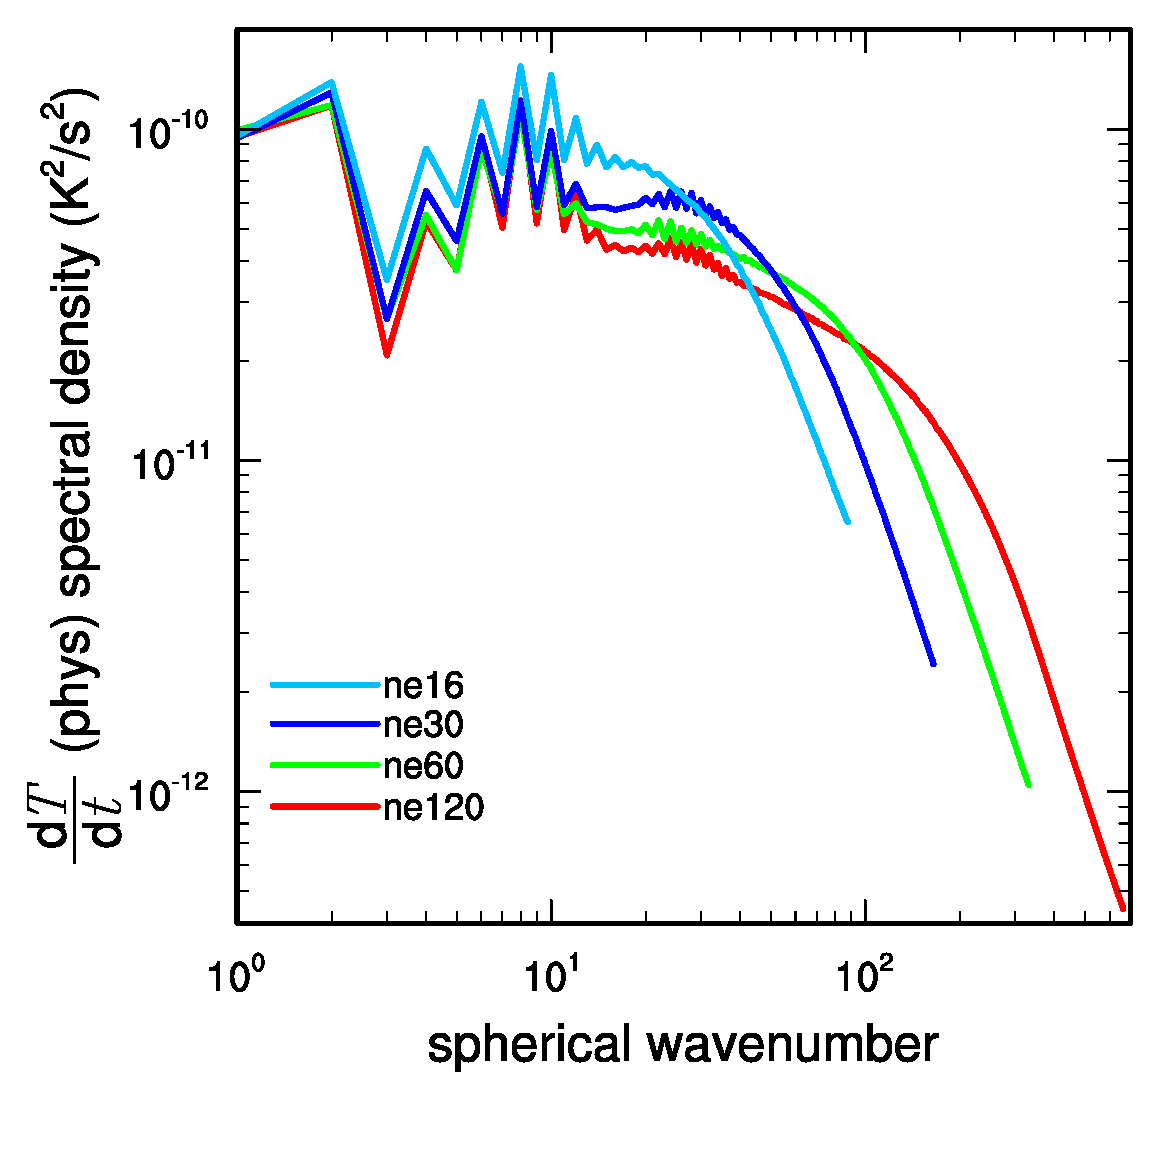
\includegraphics[width=25pc,angle=0]{chapter3/SFigure1.eps}\\
\end{center}
\caption{Global 400 hPa power spectral density of the temperature tendency arising from the CAM5 physics routines in the aqua-planet simulations.}
\label{fig:sfigure3-1}
\end{figure}

\begin{figure}
\begin{center}
\noindent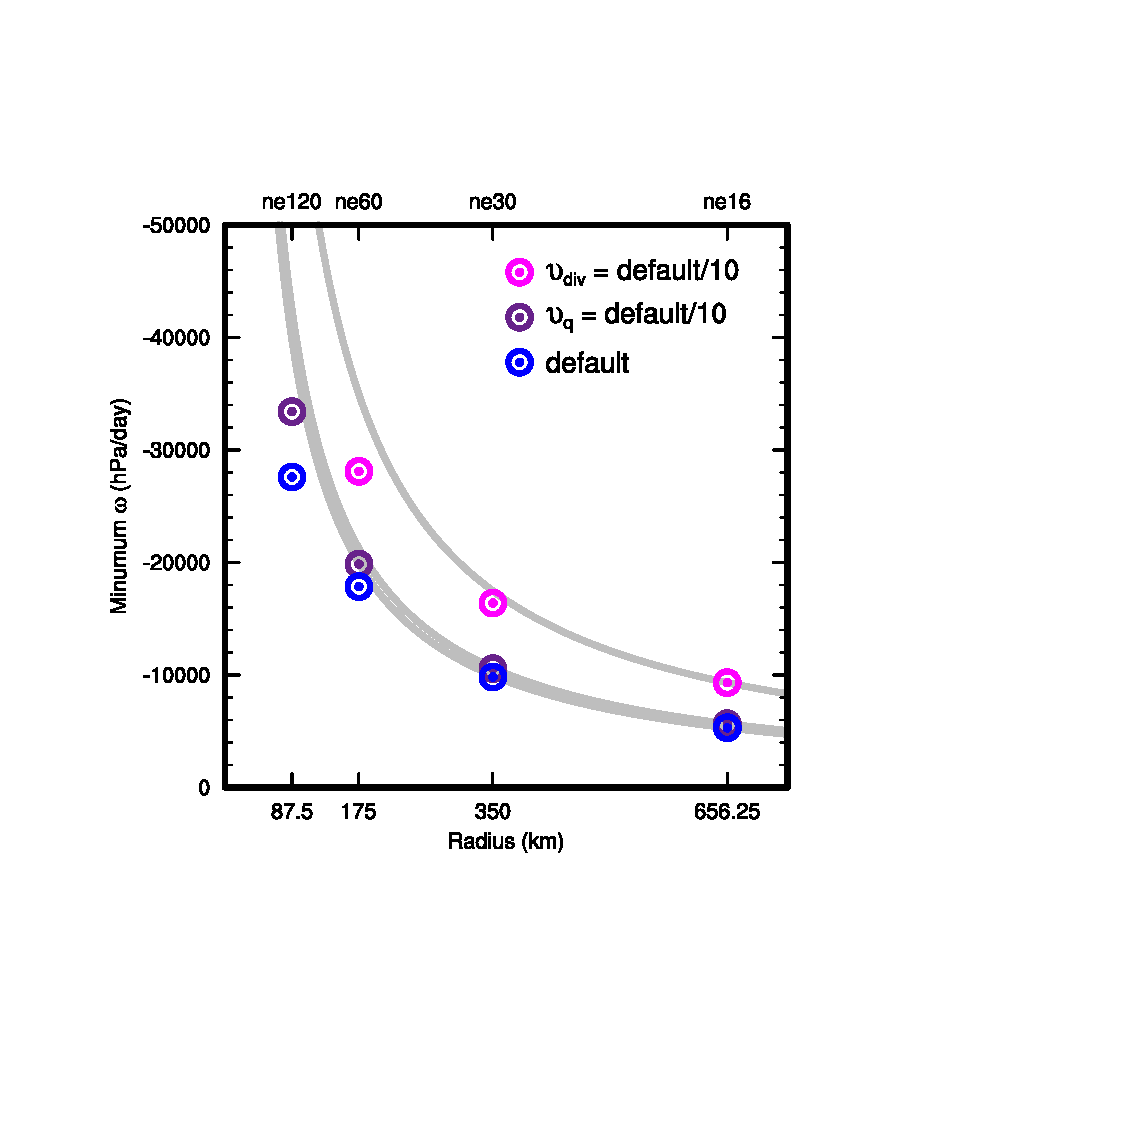
\includegraphics[width=25pc,angle=0]{chapter3/SFigure2_crop.pdf}\\
\end{center}
\caption{Results of three moist bubble experiments using CAM-SE coupled to the CAM5 stratiform scheme, using a physics time-step of 450 s. Results are expressed as the minimum vertical pressure velocity, $\omega$, over the duration of each simulation as a function of initial bubble radius. Each experiment contains four simulations, with grid-spacing (top x-axis) and initial size of the bubble (bottom x-axis) progressively decreasing. The purple markers indicate an experiment in which the specific humidity hyper-viscosity coefficient is reduced by an order of magnitude. Similarly, the pink markers denote an experiment in which the divergence damping coefficient is reduced by an order of magnitude. The highest resolution divergence damping coefficient result is not shown since this configuration resulted in model failure.}
\label{fig:sfigure3-2}
\end{figure}
